\section{CÔNG THỨC XÁC SUẤT TOÀN PHẦN -- CÔNG THỨC BAYES}
\subsection{LÝ THUYẾT CẦN NHỚ}
\vskip -0.5cm
	\immini{
	\subsubsection{Công thức xác suất toàn phần}
Cho hai biến cố $A$ và $B$ là hai biến cố tùy ý. Khi đó\\
	\boxminit{$\mathrm{P}(B)=\mathrm{P}(A)\cdot \mathrm{P}(B|A)+\mathrm{P}(\overline{A})\cdot \mathrm{P}(B|\overline{A})$}
	\subsubsection{Công thức Bayes}
	Cho hai biến cố $A$ và $B$ với $\mathrm{P}(B)>0$. Khi đó
	\boxminit{$\mathrm{P}\left(A|B\right)=\dfrac{\mathrm{P}(A)\cdot\mathrm{P}\left(B|A\right)}{\mathrm{P}(B)}$}
	Công thức Bayes còn được viết dưới dạng $$\mathrm{P}(A | B)=\dfrac{\mathrm{P}(A) \cdot \mathrm{P}(B \mid A)}{\mathrm{P}(A)\cdot \mathrm{P}(B | A)+\mathrm{P}\left(\overline{A}\right)\cdot  \mathrm{P}\left(B | \overline{A}\right)}.$$
}{\vspace{2cm}
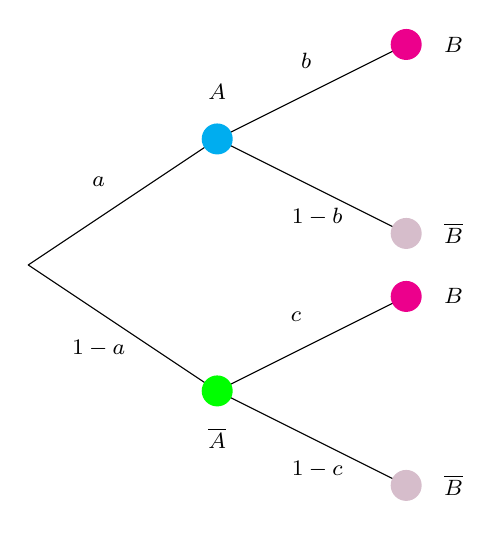
\begin{tikzpicture}[scale=0.8, font=\footnotesize, line join=round, line cap=round, >=stealth]
	\draw (0,0)--(3,2) node [midway, shift=(140:4mm)] {$a$} --(6,3.5) node [midway, shift=(100:4mm)] {$b$};
	\draw (0,0)--(3,-2) node [midway, shift=(-140:4mm)] {$1-a$} --(6,-3.5) node [midway, shift=(-80:4mm)] {$1-c$};
	\draw (3,2)--(6,0.5) node [midway, shift=(-80:4mm)] {$1-b$};
	\draw (3,-2)--(6,-0.5) node [midway, shift=(120:4mm)] {$c$};
	\draw[draw=none,fill=cyan] (3,2) circle [radius=7pt] node[shift=(90:6mm)] {$A$};
	\draw[draw=none,fill=green] (3,-2) circle [radius=7pt] node[shift=(-90:6mm)] {$\overline{A}$};
	\draw[draw=none,fill=magenta] (6,3.5) circle [radius=7pt] node[shift=(0:6mm)] {$B$};
	\draw[draw=none,fill=magenta!40!black!30] (6,0.5) circle [radius=7pt] node[shift=(0:6mm)] {$\overline{B}$};
	\draw[draw=none,fill=magenta] (6,-0.5) circle [radius=7pt] node[shift=(0:6mm)] {$B$};
	\draw[draw=none,fill=magenta!40!black!30] (6,-3.5) circle [radius=7pt] node[shift=(0:6mm)] {$\overline{B}$};
\end{tikzpicture}}
\subsection{PHÂN LOẠI VÀ PHƯƠNG PHÁP GIẢI TOÁN}
\begin{dang}{Công thức xác suất toàn phần}
\end{dang}
\boxmini{BÀI TẬP TỰ LUẬN}
\setcounter{vd}{0}
\begin{vd}%[CD, Mức độ 1]%[Trần Ngọc Thành]%[2D5H2-2]
	Cho hai biến cố $A$, $B$ với $\mathrm{P}(B)=0{,}6$; $\mathrm{P}(A|B) =0{,}7$ và $\mathrm{P}\left(A|\overline{B}\right)=0{,}4$. Tính $\mathrm{P}(A)$.
	\loigiai{
		Ta có $\mathrm{P}\left(\overline{B}\right)= 1- \mathrm{P}(B) = 1-0{,}6 = 0{,}4$.\\
		Áp dụng công thức xác suất toàn phần, ta có
		\[\mathrm{P}(A) = \mathrm{P}(A|B)\cdot \mathrm{P}(B) + \mathrm{P}\left(A|\overline{B}\right)\cdot \mathrm{P}\left(\overline{B}\right)= 0{,}7\cdot 0{,}6 + 0{,}4\cdot 0{,}4=0{,}58.\]
	}
\end{vd}
\dongcham{3}
\begin{vd}%[Mức độ 1]
	Cho hai biến cố $A$, $B$ sao cho $\mathrm{P}(A) = 0{,}6$; $\mathrm{P}(B)=0{,}4$; $\mathrm{P}(B\mid\overline{A}) = 0{,}3$. Tính~$\mathrm{P}(B|A)$.
	\loigiai{
		Áp dụng công thức xác suất toàn phần ta có	$$\mathrm{P}(B)=\mathrm{P}(A)\cdot \mathrm{P}(B \mid A)+\mathrm{P}(\overline{A}) \cdot \mathrm{P}(B \mid \overline{A}) 
		\Leftrightarrow 0{,}4=0{,}6\cdot\mathrm{P}(B \mid A) +0{,}4 \cdot 0{,}3.$$
		Suy ra $\mathrm{P}(B|A)=\dfrac{7}{15} . $}
\end{vd}
\dongcham{5}

\begin{vd}%[KNTT, Mức độ 2]%[Trần Ngọc Thành]%[2D5H2-2]
%	\immini{
		Số khán giả đến xem buổi biểu diễn ca nhạc ngoài trời phụ thuộc vào thời tiết. Giả sử, nếu trời không mưa thì xác suất để bán hết vé là $0{,}9$; còn nếu trời mưa thì xác suất để bán hết vé chỉ là $0{,}4$. Dự báo thời tiết cho thấy xác suất để trời mưa vào buổi biểu diễn là $0{,}75$. Nhà tổ chức sự kiện quan tâm đến xác suất để bán được hết vé là bao nhiêu.	
%	}{		\includegraphics[scale=0.35]{images/im2D5-2-1.png}}
	Gọi $A$ là biến cố \lq \lq Trời mưa\rq \rq~và $B$ là biến cố \lq \lq Bán hết vé\rq \rq~trong tình huống.
	\begin{enumerate}[a)]
		\item Tính $\mathrm{P}(A), \mathrm{P}(\overline{A}), \mathrm{P}(B \mid A), \mathrm{P}(B \mid \overline{A})$.
		\item Tính xác suất để nhà tổ chức sự kiện bán hết vé.
	\end{enumerate}
	\loigiai{
		\begin{enumerate}[a)]
			\item $\mathrm{P}(A)=0{,}75$; $\mathrm{P}(\overline{A})=1-\mathrm{P}(A)=0{,}25$; $\mathrm{P}(B\mid A)=0{,}4$; $\mathrm{P}(B\mid \overline{A})=0{,}9$.
			\item 	Ta có $\mathrm{P}(B)= \mathrm{P}(A) \cdot \mathrm{P}(B \mid A)+\mathrm{P}(\overline{A}) \cdot \mathrm{P}(B \mid \overline{A}) = 0{,}75\cdot 0{,}4 +0{,}25\cdot 0{,}9=0{,}525$.
	\end{enumerate}}
\end{vd}
\dongcham{7}
\begin{vd}%[KNTT, Mức độ 2]%[Trần Ngọc Thành]%[2D5H2-2]
	Trong một kì thi tốt nghiệp trung học phổ thông, một tỉnh X có $80 \%$ học sinh lựa chọn tổ hợp A00 (gồm các môn Toán, Vật lí, Hoá học). Biết rằng, nếu một học sinh chọn tổ hợp A00 thì xác suất để học sinh đó đỗ đại học là 0{,}6; còn nếu một học sinh không chọn tổ hợp A00 thì xác suất để học sinh đó đỗ đại học là 0{,}7. Chọn ngẫu nhiên một học sinh của tỉnh X đã tốt nghiệp trung học phổ thông trong kì thi trên. Tính xác suất để học sinh đó đỗ đại học.
	\loigiai{Gọi $A$ là biến cố: \lq \lq Học sinh đó chọn tổ hợp A00\rq \rq~; $B$ là biến cố: \lq \lq Học sinh đó đỗ đại học\rq \rq.\\
		Ta cần tính $\mathrm{P}(B)$. Theo công thức xác suất toàn phần, ta cần biết: $\mathrm{P}(A), \mathrm{P}(\overline{A}), \mathrm{P}(B \mid A)$ và $\mathrm{P}(B \mid \overline{A})$.\\
		Ta có: $\mathrm{P}(A)=0{,}8; \mathrm{P}(\overline{A})=1-\mathrm{P}(A)=1-0{,}8=0{,}2$.\\
		$\mathrm{P}(B \mid A)$ là xác suất để một học sinh đỗ đại học với điều kiện học sinh đó chọn tổ hợp $A 00$ \\$\Rightarrow \mathrm{P}(B \mid A)=0{,}6$.\\
		$\mathrm{P}(B \mid \overline{A})$ là xác suất để một học sinh đỗ đại học với điều kiện học sinh đó không chọn tổ hợp $\mathrm{A} 00$\\$ \Rightarrow \mathrm{P}(B \mid \overline{A})=0{,}7$.\\
		Thay vào công thức xác suất toàn phần ta được:$$\mathrm{P}( B)={\mathrm{P}(A) \cdot \mathrm{P}(B \mid A)+\mathrm{P}(\overline{A}) \cdot \mathrm{P}(B \mid \overline{A})}={0{,}8 \cdot 0{,}6+0{,}2 \cdot 0{,}7} = 0{,}62.$$}
\end{vd}
\dongcham{8}
\begin{vd}%[CD, Mức độ 2]%[Trần Ngọc Thành]%[2D5H2-2]
	Một loại linh kiện do hai nhà máy số I, số II cùng sản xuất. Tỉ lệ phế phẩm của các nhà máy I, II lần lượt là $4\%$; $3\%$. Trong một lô linh kiện để lẫn lộn $80$ sản phẩm của nhà máy số I và $120$ sản phẩm của nhà máy số II. Một khách hàng lấy ngẫu nhiên một linh liện từ lô hàng đó.
	Tính xác suất để linh kiện được lấy ra là linh kiện tốt.
	\loigiai{
		
		Xét các biến cố
		\begin{itemize}
			\item[] $A$: \lq\lq Linh kiện lấy ra là linh kiện tốt\rq\rq.
			\item[] $B$: \lq\lq Linh kiện lấy ra là linh kiện từ nhà máy số I\rq\rq.
			\item[] $\overline{B}$: \lq\lq Linh kiện lấy ra là linh kiện từ nhà máy số II\rq\rq.
		\end{itemize}
		Theo đề bài, ta có
		\begin{listEX}[2]
			\item[] $\mathrm{P}(A|B) =1 - 0{,}04 = 0{,}96$.
			\item[] $\mathrm{P}\left(A|\overline{B}\right) = 1-0{,}03 = 0{,}97$.
			\item[] $\mathrm{P}(B)=\dfrac{80}{200}=0{,}4$.
			\item[] $\mathrm{P}\left(\overline{B}\right) = \dfrac{120}{200}=0{,}6$.
		\end{listEX}
		Khi đó áp dụng công thức xác suất toàn phần, ta có
		\[\mathrm{P}(A) = \mathrm{P}(A|B)\cdot \mathrm{P}(B) + \mathrm{P}\left(A|\overline{B}\right)\cdot\mathrm{P}\left(\overline{B}\right)=0{,}96\cdot 0{,}4 + 0{,}97\cdot 0{,}6=0{,}966.\]		
	}
\end{vd}
\dongcham{8}


\begin{vd}%[KNTT, Mức độ 3]%[Trần Ngọc Thành]%[2D5H2-2]%[2D5H2-2]
	Tại nhà máy X sản xuất linh kiện điện tử tỉ lệ sản phẩm đạt tiêu chuẩn là $80 \%$. Trước khi xuất xưởng ra thị trường, các linh kiện điện tử đều phải qua khâu kiểm tra chất lượng để đóng dấu OTK. Vì sự kiểm tra không tuyệt đối hoàn hảo nên nếu một linh kiện điện tử đạt tiêu chuẩn thì nó có xác suất $ 0{,}99 $ được đóng dấu OTK; nếu một linh kiện điện tử không đạt tiêu chuẩn thì nó có xác suất $ 0{,}95 $ không được đóng dấu OTK. Chọn ngẫu nhiên một linh kiện điện tử của nhà máy X trên thị trường.
	\begin{enumerate}[a)]
		\item Tính xác suất để linh kiện điện tử đó được đóng dấu OTK.
		\item Tính xác suất để linh kiện điện tử đó không được đóng dấu OTK.
	\end{enumerate}

	\loigiai{Gọi $A$ là biến cố: \lq \lq Linh kiện điện tử đó đạt tiêu chuẩn\rq \rq~. Gọi $B$ là biến cố: \lq \lq Linh kiện điện tử đó được đóng dấu OTK\rq \rq~.
		\begin{enumerate}[a)]
			\item Ta có $\mathrm{P}(B)=\mathrm{P}(A)\cdot \mathrm{P}(B \mid A)+\mathrm{P}(\overline{A}) \cdot \mathrm{P}(B \mid \overline{A})$.
			\begin{itemize}
				\item Tính $\mathrm{P}(A)$: Đây là xác suất để linh kiện đó đạt tiêu chuẩn. Vậy $\mathrm{P}(A)=0{,}8$.
				\item Tính $\mathrm{P}(\overline{A})$: $\mathrm{P}(\overline{A})=1-\mathrm{P}(A)=0{,}2$.
				\item Tính $\mathrm{P}(B\mid A)$: Đây là xác suất để linh kiện điện tử đó được đóng dấu OTK với điều kiện nó đạt tiêu chuẩn. Vậy $\mathrm{P}(B\mid A)=0{,}99$.
				\item Tính $\mathrm{P}(B\mid \overline{A})$: Đây là xác suất để linh kiện điện tử đó được đóng dấu OTK với điều kiện nó không đạt tiêu chuẩn. Vậy $\mathrm{P}(B\mid \overline{A})=1-0{,}95=0{,}05$.
			\end{itemize}
			Vậy $\mathrm{P}(B)=\mathrm{P}(A)\cdot \mathrm{P}(B \mid A)+\mathrm{P}(\overline{A}) \cdot \mathrm{P}(B \mid \overline{A})=0{,}8\cdot 0{,}99+0{,}2\cdot 0{,}05=0{,}802$. \\
			Vậy xác suất để  linh kiện điện tử đó được đóng dấu OTK là $0{,}802$.
			\item Ta có sơ đồ hình cây
			\begin{center}
				\begin{tikzpicture}[scale=0.8, font=\footnotesize, line join=round, line cap=round, >=stealth]
					\draw (0,0)--(-2,-2.5) node [midway, shift=(140:4mm)] {$0{,}8$} --(-3,-5) node [midway, shift=(160:4mm)] {$0{,}99$};
					\draw (0,0)--(2,-2.5) node [midway, shift=(40:4mm)] {$0{,}2$} --(3,-5) node [midway, shift=(20:4mm)] {$0{,}95$};
					\draw (-2,-2.5)--(-1,-5) node [midway, shift=(20:4mm)] {$0{,}01$};
					\draw (2,-2.5)--(1,-5) node [midway, shift=(160:4mm)] {$0{,}05$};
					\draw[draw=none,fill=yellow] (0,0) circle [radius=7pt] node[shift=(90:6mm)] {Gốc $O$};
					\draw[draw=none,fill=cyan] (-2,-2.5) circle [radius=7pt] node[shift=(140:6mm)] {$A$};
					\draw[draw=none,fill=green] (2,-2.5) circle [radius=7pt] node[shift=(40:6mm)] {$\overline{A}$};
					\draw[draw=none,fill=magenta] (1,-5) circle [radius=7pt] node[shift=(-90:6mm)] {$B$};
					\draw[draw=none,fill=magenta!40!black!30] (-1,-5) circle [radius=7pt] node[shift=(-90:6mm)] {$\overline{B}$};
					\draw[draw=none,fill=magenta] (-3,-5) circle [radius=7pt] node[shift=(-90:6mm)] {$B$};
					\draw[draw=none,fill=magenta!40!black!30] (3,-5) circle [radius=7pt] node[shift=(-90:6mm)] {$\overline{B}$};
				\end{tikzpicture}
			\end{center}
			Có hai nhánh cây đi từ $O$ tới $\overline{B}$ là $OA\overline{B}$ và $O\overline{A}\cdot\overline{B}$. Vậy xác suất để linh kiện điện tử được chọn không được đóng dấu OTK là $$\mathrm{P}(\overline{B})=0{,}8\cdot 0{,}01+0{,}2\cdot 0{,}95=0{,}198.$$
		\end{enumerate}
	}
\end{vd}
\dongcham{8}
\begin{vd}%[CTST, Mức độ 3]%[Trần Ngọc Thành]%[2D5V2-2]%[2D5V2-4]
	Hộp thứ nhất có $1$ viên bi xanh và $5$ viên bi đỏ. Hộp thứ hai có $3$ viên bi xanh và $5$ viên bi đỏ. Các viên bi có cùng kích thước và khối lượng. Lấy ra ngẫu nhiên đồng thời $2$ viên bi từ hộp thứ nhất chuyển sang hộp thứ hai. Sau đó lại lấy ra ngẫu nhiên $2$ viên bi từ hộp thứ hai.
	Tính xác suất để hai viên bi lấy ra từ hộp thứ hai là bi đỏ.
	\loigiai{
		Xét các biến cố
		\begin{itemize}
			\item $A$: \lq\lq Hai viên bi lấy ra từ hộp thứ hai là bi đỏ\rq\rq.
			\item $B_1$: \lq\lq Hai viên bi lấy ra từ hộp thứ nhất có cả màu xanh và màu đỏ\rq\rq. 
			\item $B_2$: \lq\lq Hai viên bi lấy ra từ hộp thứ nhất có màu đỏ\rq\rq.
		\end{itemize}
		Ta có 
		\[\mathrm{P}(B_1) = \dfrac{\mathrm{C}^1_{5}}{\mathrm{C}^2_{6}}=\dfrac{1}{3};\quad 
		\mathrm{P}(B_2) = \dfrac{\mathrm{C}^2_5}{\mathrm{C}^2_{6}}=\dfrac{2}{3};\quad
		\mathrm{P}(A\mid B_1) = \dfrac{\mathrm{C}^2_6}{\mathrm{C}^2_{10}}=\dfrac{1}{3};\quad
		\mathrm{P}(A\mid B_2) = \dfrac{\mathrm{C}^2_7}{\mathrm{C}^2_{10}}=\dfrac{7}{15}.
		\]
		Áp dụng công thức xác suất toàn phần, ta có
		\allowdisplaybreaks
		\begin{eqnarray*}
			\mathrm{P}(A) 
			&=& \mathrm{P}(A|B_1)\cdot \mathrm{P}(B_1) + \mathrm{P}(A|B_2)\cdot\mathrm{P}(B_2)\\ 
			&=& \dfrac{1}{3}\cdot \dfrac{1}{3} + \dfrac{7}{15}\cdot \dfrac{2}{3}\\
			&=& \dfrac{19}{45}.
		\end{eqnarray*}
		
}\end{vd}
\dongcham{8}
\begin{vd}
	Trong trò chơi hái hoa có thưởng của lớp 12A, cô giáo treo $10$ bông hoa trên cành cây, trong đó có $5$ bông hoa chứa phiếu có thưởng. Bạn Bình hái bông hoa đầu tiên, sau đó bạn An hái bông hoa thứ hai. Tính xác suất bạn An hái được bông hoa chứa phiếu có thưởng.
	\loigiai{
		Xét hai biến cố
		\begin{itemize}
			\item[] $A$: \lq\lq Bông hoa bạn An hái được chứa phiếu có thưởng\rq\rq.
			\item[] $B$: \lq\lq Bông hoa bạn Bình hái được chứa phiếu có thưởng\rq\rq. 
		\end{itemize}
		Khi đó, ta có
		\begin{listEX}[3]
			\item[] $\mathrm{P}(B)=\dfrac{5}{10}=\dfrac{1}{2}$
			\item*[] $\mathrm{P}\left(\overline{B}\right) = 1 - \mathrm{P}(B)=1-\dfrac{1}{2}=\dfrac{1}{2}$
			\item[] $\mathrm{P}(A|B)=\dfrac{4}{9}$
			\item*[] $\mathrm{P}\left(A|\overline{B}\right)=\dfrac{5}{9}$.
		\end{listEX}
		\begin{enumerate}
			\item Sơ đồ hình cây biểu thị tình huống đã cho là
			\begin{center}
				\begin{tikzpicture}[->,>=stealth,line join=round,line cap=round,font=\footnotesize,scale=1]
					\def\xmot{3}
					\def\xhai{8}
					\node (O) at (0,0){};
					\node (B) at (\xmot,1){$B$};
					\node (B1) at (\xmot,-1){$\overline{B}$};
					\node (BA) at (\xhai,2){$A$};
					\node (BA1) at (\xhai,0.3){$\overline{A}$};
					\node (B1A) at (\xhai,-0.3){$A$};
					\node (B1A1) at (\xhai,-1.75){$\overline{A}$};
					
					\foreach \x/\y/\p/\l in 
					{
						O/B/above/$\mathrm{P}(B)=\dfrac{1}{2}$,
						B/BA/above/$\mathrm{P}(A|B)=\dfrac{4}{9}$,
						B/BA1//,
						O/B1/below/$\mathrm{P}\left(\overline{B}\right)=\dfrac{1}{2}$,
						B1/B1A/above/$\mathrm{P}\left(A|\overline{B}\right)=\dfrac{5}{9}$,
						B1/B1A1//
					}
					{
						\draw[->] (\x)--(\y)node[midway,\p,scale=0.8,sloped]{\l};
					}
					\node (mot) at (\xmot,4) {Bông hoa bạn Bình hái ra};
					\node (hai) at (\xhai,4) {Bông hoa bạn An hái ra};
					\draw[->,thick,orange] (mot)--(B);
					\draw[->,thick,orange] (hai)--(BA);
				\end{tikzpicture}
			\end{center}
			\item Áp dụng công thức tính xác suất toàn phần, ta có:
			\[\mathrm{P}(A) = \mathrm{P}(B)\cdot\mathrm{P}\left(A|B\right) + \mathrm{P}\left(\overline{B}\right)\cdot\mathrm{P}\left(A|\overline{B}\right) = \dfrac{1}{2}\cdot \dfrac{4}{9} + \dfrac{1}{2}\cdot\dfrac{5}{9}=\dfrac{1}{2}.\]
			Vậy xác suất bạn An hái được bông hoa chứa phiếu có thưởng bằng $\dfrac{1}{2}$.
		\end{enumerate}
	}
\end{vd}

\dongcham{8}

\boxmini{BÀI TẬP TRẮC NGHIỆM}
\setcounter{ex}{0}
\Opensolutionfile{ans}[ans/2D6-B2-d1-1]

\begin{ex}%[KNTT, Mức độ 1]%[Trần Ngọc Thành]%[2D5H2-2]
	Cho $\mathrm{P}(A)=\dfrac{2}{5}$; $\mathrm{P}\left( B\mid A\right)=\dfrac{1}{3}$; $\mathrm{P}\left(B\mid \overline{A}\right)=\dfrac{1}{4}$. Giá trị của $\mathrm{P}(B)$ là 
	\choice
	{$\dfrac{19}{60} $}
	{\True $ \dfrac{17}{60}$}
	{$ \dfrac{9}{20}$}
	{$ \dfrac{7}{30}$}
	\loigiai{Áp dụng công thức xác suất toàn phần ta có
		
		$\mathrm{P}(B)=\mathrm{P}(A)\cdot \mathrm{P}(B\mid A)+\mathrm{P}\left( \overline{A}\right) \cdot \mathrm{P}\left( B\mid \overline{A}\right)=\dfrac{2}{5}\cdot \dfrac{1}{3}+\dfrac{3}{5}\cdot \dfrac{1}{4}=\dfrac{17}{60}$.
	}
\end{ex}\cham{2}
\begin{ex}%[CD, Mức độ 1]%[Trần Ngọc Thành]%[2D5H2-2]
	Cho hai biến cố $A$, $B$ với $\mathrm{P}(B)=0{,}6$; $\mathrm{P}(A|B) =0{,}7$ và $\mathrm{P}\left(A|\overline{B}\right)=0{,}4$. Khi đó, $\mathrm{P}(A)$ bằng
	\choice
	{$0{,}7$}
	{$0{,}4$}
	{\True $0{,}58$}
	{$0{,}52$}
	\loigiai{
		Ta có $\mathrm{P}\left(\overline{B}\right)= 1- \mathrm{P}(B) = 1-0{,}6 = 0{,}4$.\\
		Áp dụng công thức xác suất toàn phần, ta có
		\[\mathrm{P}(A) = \mathrm{P}(A|B)\cdot \mathrm{P}(B) + \mathrm{P}\left(A|\overline{B}\right)\cdot \mathrm{P}\left(\overline{B}\right)= 0{,}7\cdot 0{,}6 + 0{,}4\cdot 0{,}4=0{,}58.\]
	}
\end{ex}\cham{2}
\begin{ex}%[CKP, Mức độ 2]%[Trần Ngọc Thành]%[2D5H2-2]
	Cho $A$, $B$ là các biến cố thỏa mãn $P\left( {\overline {A}\cdot\overline {B} } \right)=0{,}35$, $\mathrm{P}(A)=0{,}25$, $\mathrm{P}\left( B\mid A\right)=0{,}8$. 
	Giá trị của $\mathrm{P}(B)$ bằng
	\choice
	{$\dfrac{1}{5}$}
	{\True$\dfrac{3}{5}$}
	{$\dfrac{7}{15}$}
	{$\dfrac{2}{3}$}
	\loigiai{Ta có $P\left( {\overline {A}\cdot\overline {B} } \right) = P\left( {\overline A } \right)P\left( {\overline B |\overline A } \right) \Rightarrow P\left( {\overline B |\overline A } \right) = \dfrac{{P\left( {\overline {A}\cdot\overline {B} } \right)}}{{P\left( {\overline A } \right)}} = \dfrac{{0{,}35}}{{0{,}75}} = \dfrac{7}{{15}}.$ \\
		Suy ra $P\left( {B|\overline A } \right) = 1 - \dfrac{7}{{15}} = \dfrac{8}{{15}}$.\\
		Theo công thức xác suất toàn phần, ta có
		$$\begin{array}{l}
			P\left( B \right) = P\left( {B|A} \right)P\left( A \right) + P\left( {B|\overline A } \right)P\left( {\overline A } \right)=\dfrac{3}{5}.
		\end{array}.$$
	}
\end{ex}\cham{2}

%Bt 6.18
\begin{ex}%[CTST, Mức độ 2]%[Trần Ngọc Thành]%[2D5Y2-3]
	Tỉ lệ người dân đã tiêm vắc xin phòng bệnh A ở một địa phương là $65\%$. Trong số những 
	người đã tiêm phòng, tỉ lệ mắc bệnh A là $5\%$ còn trong số những người chưa tiêm, tỉ lệ 
	mắc bệnh A là $17\%$. Gặp ngẫu nhiên một người ở địa phương đó.
	Xác suất người đó mắc bệnh A là
	\choice
	{$0{,}0325$}
	{$0{,}018$}
	{\True $0{,}092$}
	{$0{,}0525$}
	\loigiai{Gọi $H_1$ là biến cố \lq \lq Gặp được người đã tiêm vắc xin phòng bệnh $A$\rq \rq , $H_2$ là biến cố \lq \lq Gặp được người chưa tiêm vắc xin phòng bệnh $A$\rq \rq , $K$ là biến cố \lq \lq  người đó mắc bệnh A\rq \rq .	
		Theo công thức xác suất toàn phần, ta có:
		$$\mathrm{P}(K)=\mathrm{P}(H_1).\mathrm{P}(K|H_1)+\mathrm{P}(H_2).\mathrm{P}(K|H_2)$$
		$$ \Leftrightarrow \mathrm{P}(K)= 0{,}65.0{,}05+0{,}35.0{,}17=0{,}092. $$
		
	}
\end{ex}\cham{3}
\begin{ex}%[CTST, Mức độ 2]%[BG12-4in1, Trần Ngọc Thành]%[ID6]
	Một nhà máy có hai phân xưởng I và II. Phân xưởng I sản xuất $40\%$ số sản phẩm 
	và phân xưởng II sản xuất $60\%$ số sản phẩm. Tỉ lệ sản phẩm bị lỗi của phân xưởng I 	là $2\%$ và của phân xưởng II là $1\%$. Kiểm tra ngẫu nhiên 1 sản phẩm của nhà máy và xác suất để sản phẩm đó bị lỗi là
	\choice
	{$0{,}02$}
	{$0{,}6$}
	{\True $0{,}014$}
	{$0{,}01$}
	\loigiai{
		Gọi $A$ là biến cố “Sản phẩm bị lỗi” và $B$ là biến cố “Sản phẩm lấy ra do phân xưởng I 
		sản xuất”.\\
		Do phân xưởng I sản xuất $40\%$ số sản phẩm và phân xưởng II sản xuất $60\%$ số sản phẩm nên
		$$\mathrm{P}(B)=0{,}4 \text{ và } \mathrm{P}(\overline{B})=1-0{,}4=0{,}6.$$
		Do tỉ lệ sản phẩm bị lỗi của phân xưởng I là $2\%$ và của phân xưởng II là $1\%$ nên
		$$\mathrm{P}(A|B)=0{,}02 \text{ và } \mathrm{P}(A|\overline{B})=1-0{,}01.$$
		Xác suất để sản phẩm lấy ra bị lỗi là
		$$\mathrm{P}(A)=\mathrm{P}(B)\mathrm{P}(A|B)+\mathrm{P}(\overline{B})\mathrm{P}(A|\overline{B})=0{,}4\cdot0{,}02+0{,}6 \cdot 0{,}01=0{,}014.$$
	}
\end{ex}\cham{3}
\begin{ex}%[CKP, Mức độ 2]%[Trần Ngọc Thành]%[2D5H2-2]
	Kết quả khảo sát tại một xã cho thấy có $20 \%$ cư dân hút thuốc lá. Tỉ lệ cư dân thường xuyên gặp các vấn đề sức khoẻ về đường hô hấp trong số những người hút thuốc lá và không hút thuốc lá lần lượt là $70\%$, $15\%$.
	Tỉ lệ gặp một cư dân của xã thì xác suất người đó thường xuyên gặp các vấn đề sức khoẻ về đường hô hấp là bao nhiêu phần trăm?
	\choice
	{\True $26\%$}
	{$12\%$}
	{$68\%$}
	{$24\%$}
	\loigiai{
		Giả sử ta gặp một cư dân của xã, gọi $A$ là biến cố \lq\lq Người đó có hút thuốc lá\rq\rq\, và $B$ là biến cố \lq\lq Người đó thường xuyên gặp các vấn đề sức khoẻ về đường hô hấp\rq\rq. Ta có sơ đồ hình cây sau.
		\begin{center}
			\begin{tikzpicture}[scale=.3,>=stealth,every node/.style={shape=rectangle,draw,rounded corners, color=blue, fill=blue!10}]
				%-------------
				\tikzstyle{block} = [rectangle, draw, fill=blue!10, rounded corners, text centered, text width = 10em, minimum height = 2em]
				%-------------
				\node (c1) {Gặp một cư dân};
				\node (c2) [above right = 2cm of c1]{$A$};
				\node (c3) [ below right= 2cm of c1]{$\overline{A}$};
				\node (c4) [above right = 1cm of c2]{$B$} ;
				\node (c5) [below right = 1cm of c2]{$\overline{B}$};
				\node (c6) [ above right =1cm of c3]{$B$};
				\node (c7) [ below right = 1cm of c3]{$\overline{B}$};
				%--------------
				\draw 
				(17.5,15) node[right] {\text{Kết quả}} 
				(20,11.3) node[right] {$AB$} 
				(20,2.5) node[right] {$A\overline{B}$} 
				(20,-2.5) node[right] {$\overline{A}B$} 
				(20,-11.5) node[right] {$\overline{A}\cdot\overline{B}$};
				%--------------
				\draw 
				(25,15) node[right] {\text{Xác suất}} 
				(25,11.3) node[right] {$0{,}14$} 
				(25,2.5) node[right] {$0{,}06$} 
				(25,-2.5) node[right] {$0{,}12$} 
				(25,-11.5) node[right] {$0{,}68$};
				%------------
				\draw[->] (c1.east) --node[above left]{$0{,}2$} (c2.west);
				\draw[->] (c1.east) --node[below left]{$0{,}8$} (c3.west);
				\draw[->] (c2.east) --node[above left]{$0{,}7$} (c4.west);
				\draw[->] (c2.east) --node[below left]{$0{,}3$} (c5.west);
				\draw[->] (c3.east) --node[above left]{$0{,}15$} (c6.west);
				\draw[->] (c3.east) -- node[below left]{$0{,}85$} (c7.west);
			\end{tikzpicture}
		\end{center}
		Ta có $\mathrm{P}(B)=\mathrm{P}(A) \cdot \mathrm{P}(B | A)+\mathrm{P}(\overline{A}) \cdot \mathrm{P}\left(B | \overline{A}\right)=0{,}14+0{,}12=0{,}26$.\\
		Vậy nếu ta gặp một cư dân của xã thì xác suất người đó thường xuyên gặp các vấn đề sức khoẻ về đường hô hấp là $26\%$.
	}
\end{ex}\cham{3}


\begin{ex}%[CKP, Mức độ 2]%[Trần Ngọc Thành]%[2D5H2-2]
	Một bệnh viện có hai phòng khám là phòng A và phòng B với khả năng lựa chọn của bệnh nhân là như nhau. Tỉ lệ bệnh nhân nam có ở phòng A và phòng B lần lượt là $60\%$ và $40\%$. Một người bệnh được chọn ngẫu nhiêu từ hai phòng khám .Tính xác suất để người bệnh được chọn người này là nam là
	\choice
	{ $0{,}6$}
	{\True $0{,}5$}
	{$0{,}4$}
	{$0{,}3$}
	\loigiai{Một người bệnh được chọn ngẫu nhiên từ hai phòng khám.\\
		Gọi $X$ là biến cố \lq \lq Người đó đến từ phòng khám A\rq \rq \, và $Y$, $\overline{Y}$ lần lượt là biến cố \lq \lq Người đó là nam\rq \rq \; và \lq \lq Người đó không là nam\rq \rq.\\
		Ta có sơ đồ hình cây sau\\
		\begin{tikzpicture}[>=stealth]
			%Khung 1
			\draw (-2,-1) rectangle (2.2,0);
			\draw (0.1,-0.5) node{Bệnh nhân được chọn} ;
			%Mui ten 1,2
			\draw [->] (2.2,-0.5)--(3.8,1.6) node[pos=0.5,sloped,above]{$0{,}5$};
			\draw [->] (2.2,-0.5)--(3.8,-2.6) node[pos=0.5,sloped,below]{$0{,}5$};
			%Khung 2.1
			\draw (3.8,1.1) rectangle (5.1,2.1);
			\draw (8.9/2,1.6) node{$X$} ;
			%Khung 2.2
			\draw (3.8,-2.1) rectangle (5.1,-3.1);
			\draw (8.9/2,-2.6) node{$\overline{X}$} ;
			%Mui ten 3,4
			\draw [->] (5.1,1.6)--(6.5,2.6) node[pos=0.5,sloped,above]{$0{,}6$};
			\draw [->] (5.1,1.6)--(6.5,0.6) node[pos=0.5,sloped,below]{$0{,}4$};
			%Mui ten 5,6
			\draw [->] (5.1,-2.6)--(6.5,-1.6) node[pos=0.5,sloped,above]{$0{,}4$};
			\draw [->] (5.1,-2.6)--(6.5,-3.6) node[pos=0.5,sloped,below]{$0{,}6$};
			%Khung 3.1
			\draw (6.5,2.2) rectangle (7.7,3.2);
			\draw (7.1,5.4/2) node{$Y$} ;
			%Khung 3.2
			\draw (6.5,1.2) rectangle (7.7,0.2);
			\draw (7.1,1.4/2) node{$\overline{Y}$} ;
			%Khung 3.3
			\draw (6.5,-1.1) rectangle (7.7,-2.1);
			\draw (7.1,-3.2/2) node{$Y$} ;
			%Khung 3.3
			\draw (6.5,-2.9) rectangle (7.7,-3.9);
			\draw (7.1,-3.4) node{$\overline{Y}$} ;
			%Kết quả
			\draw (9.5,3.7) node{\textbf{Kết quả}};	
			\draw (9.5,2.7) node{$XY$};
			\draw (9.5,0.7) node{$X \overline{Y}$};
			\draw (9.5,-1.6) node{$\overline{X}Y$};
			\draw (9.5,-3.4) node{$\overline{X}\cdot\overline{Y}$};
			%Xác suất
			\draw (12.5,3.7) node{\textbf{Xác suất}};	
			\draw (12.5,2.7) node{$0{,}3$};
			\draw (12.5,0.7) node{$0{,}2$};
			\draw (12.5,-1.6) node{$0{,}2$};
			\draw (12.5,-3.4) node{$0{,}3$};	
		\end{tikzpicture}
		
		Theo công thức xác suất toàn phần, ta có
		$$\mathrm{P}(Y)={\mathrm{P}(X)\mathrm{P}(Y|X)+\mathrm{P}(\overline{X})\mathrm{P}(Y|\overline{X})}={0{,}3+0{,}2}=0{,}5.$$
		Vậy với một người bệnh được chọn ngẫu nhiêu từ hai phòng khám xác suất người này là nam là $0{,}5$.}
\end{ex}\cham{6}

\begin{ex}
	Có $2$ xạ thủ loại I và $8$ xạ thủ loại II, xác suất bắn trúng đích của các loại xạ thủ loại I là $0,9$ và loại II là $0,7$. Chọn ngẫu nhiên ra một xạ thủ và xạ thủ đó bắn một viên đạn. Tìm xác suất để viên đạn đó trúng đích.
	\choice
	{\True $0,74$}
	{$0,86$}
	{$0,56$}
	{$0,68$}
	\loigiai{
		Gọi $A$ là biến cố ``Viên đạn trúng đích''; $B$ là biến cố ``Chọn xạ thủ loại I bắn''.
		
		Ta có: 
		$$P(B) = \dfrac{2}{10} = 0,2; \quad P(A|B) = 0,9; \quad P(\overline{B}) = 1 - 0,2 = 0,8; \quad P(A|\overline{B}) = 0,7$$
		
		Theo công thức xác suất thành phần ta có:
		$$P(A) = P(B)P(A|B) + P(\overline{B})P(A|\overline{B}) = 0,2 \cdot 0,9 + 0,8 \cdot 0,7 = 0,74.$$
	}
\end{ex}
\cham{6}

\begin{ex}%[CKP, Mức độ 3]%[Trần Ngọc Thành]%[2D5H2-2]
	Ở một địa phương $X$, xác suất để một người lớn trên $40$ tuổi mắc bệnh ung thư là $0{,}05$. Xác suất bác sĩ chẩn đoán đúng một người mắc bệnh ung thư là $0{,}78$ và chẩn đoán sai (không bị ung thư nhưng được chẩn đoán mắc bệnh) là $0{,}06$. Xác suất để một người nhận được kết quả chẩn đoán không bị ung thư bằng
	\choice
	{$0{,}40625$}
	{$0{,}096$}
	{\True $0{,}904$}
	{$0{,}59375$}
	\loigiai{Một bệnh nhân trên 40 tuổi ở địa phương X đến bác sĩ để khám bệnh ung thư.\\
		Gọi $A$ là biến cố \lq \lq Người đó mắc bệnh ung thư\rq \rq \, và $B$, $\overline{B}$ lần lượt là biến cố \lq \lq Bác sĩ chẩn đoán người đó bị ung thư\rq \rq \;và \lq \lq Bác sĩ chẩn đoán người đó không bị ung thư\rq \rq.\\
		Ta xét sơ đồ hình cây như sau\\
		\begin{tikzpicture}[>=stealth]
			%Khung 1
			\draw (-3.5,-1) rectangle (2.2,0);
			\draw (-1.3/2,-0.5) node{Bệnh nhân được chẩn đoán} ;
			%Mui ten 1,2
			\draw [->] (2.2,-0.5)--(3.8,1.6) node[pos=0.5,sloped,above]{$0{,}05$};
			\draw [->] (2.2,-0.5)--(3.8,-2.6) node[pos=0.5,sloped,below]{$0{,}95$};
			%Khung 2.1
			\draw (3.8,1.1) rectangle (5.1,2.1);
			\draw (8.9/2,1.6) node{$A$} ;
			%Khung 2.2
			\draw (3.8,-2.1) rectangle (5.1,-3.1);
			\draw (8.9/2,-2.6) node{$\overline{A}$} ;
			%Mui ten 3,4
			\draw [->] (5.1,1.6)--(6.5,2.6) node[pos=0.5,sloped,above]{$0{,}78$};
			\draw [->] (5.1,1.6)--(6.5,0.6) node[pos=0.5,sloped,below]{$0{,}22$};
			%Mui ten 5,6
			\draw [->] (5.1,-2.6)--(6.5,-1.6) node[pos=0.5,sloped,above]{$0{,}06$};
			\draw [->] (5.1,-2.6)--(6.5,-3.6) node[pos=0.5,sloped,below]{$0{,}94$};
			%Khung 3.1
			\draw (6.5,2.2) rectangle (7.7,3.2);
			\draw (7.1,5.4/2) node{$B$} ;
			%Khung 3.2
			\draw (6.5,1.2) rectangle (7.7,0.2);
			\draw (7.1,1.4/2) node{$\overline{B}$} ;
			%Khung 3.3
			\draw (6.5,-1.1) rectangle (7.7,-2.1);
			\draw (7.1,-3.2/2) node{$B$} ;
			%Khung 3.3
			\draw (6.5,-2.9) rectangle (7.7,-3.9);
			\draw (7.1,-3.4) node{$\overline{B}$} ;
			%Kết quả
			\draw (9.5,3.7) node{\textbf{Kết quả}};	
			\draw (9.5,2.7) node{$AB$};
			\draw (9.5,0.7) node{$A\overline{B}$};
			\draw (9.5,-1.6) node{$\overline{A}B$};
			\draw (9.5,-3.4) node{$\overline{A}\cdot\overline{B}$};
			%Xác suất
			\draw (12.5,3.7) node{\textbf{Xác suất}};	
			\draw (12.5,2.7) node{$0{,}039$};
			\draw (12.5,0.7) node{$0{,}011$};
			\draw (12.5,-1.6) node{$0{,}057$};
			\draw (12.5,-3.4) node{$0{,}893$};
		\end{tikzpicture}
		
		Theo công thức Bayes, ta có $$\mathrm{P}(B)={\mathrm{P}(A)\mathrm{P}(B|A)+\mathrm{P}(\overline{A})\mathrm{P}(B|\overline{A})}={0{,}039+0{,}057}=0{,}096.$$		 
		Suy ra $ \mathrm{P}(\overline{B})=1 - \mathrm{P}(B) =0{,}904$
		
		Xác suất để một người nhận được kết quả chẩn đoán không bị ung thư $0{,}904$.}
\end{ex}\cham{5} 
\begin{ex}%[CKP, Mức độ 3]%[Trần Ngọc Thành]%[2D5H2-2]
	Một hộp có $5$ quả cầu trắng và $10$ quả cầu đen cùng kích thước và khối lượng. Lấy ngẫu nhiên lần lượt hai quả cầu (không hoàn lại) từ hộp. Xác suất để lần thứ hai lấy được quả cầu trắng là
	\choice
	{$\dfrac{2}{3}$}
	{$\dfrac{2}{7}$}
	{$\dfrac{5}{7}$}
	{\True $\dfrac{1}{3}$}
	\loigiai{
		Xét phép thử lấy ngẫu nhiên lần lượt hai quả cầu (không hoàn lại) từ hộp. Gọi:
		\begin{itemize}
			\item $A$ là biến cố \lq \lq Lần thứ hai lấy được quả cầu trắng\rq \rq~;
			\item $B$ là biến cố \lq \lq Lần thứ nhất lấy được quả cầu trắng\rq \rq~;
			\item$\overline{B}$ là biến cố \lq \lq Lần thứ nhất lấy được quả cầu đen\rq \rq~.
		\end{itemize}
		Ta có: 
		$$\mathrm{P}(B)=\dfrac{5}{15}=\dfrac{1}{3};\quad \mathrm{P}(\overline{B})=\dfrac{10}{15}=\dfrac{2}{3}.$$
		Nếu lần thứ nhất lấy được quả cầu trắng thì trong hộp còn $4$ quả cầu trắng và $10$ quả cầu đen. Do đó $\mathrm{P}(A|B)=\dfrac{4}{14}=\dfrac{2}{7}$.\\
		Nếu lần thứ nhất lấy được quả cầu đen thì trong hộp còn $5$ quả cầu trắng và $9$ quả cầu đen. Do đó $\mathrm{P}(A|\overline{B})=\dfrac{5}{14}$.\\
		Áp dụng công thức xác suất toàn phần, ta có:
		$$\mathrm{P}(A) = \mathrm{P}(B)\cdot \mathrm{P}(A|B) + \mathrm{P}(\overline{B})\cdot \mathrm{P}(A|\overline{B}) =\dfrac{1}{3}\cdot \dfrac{2}{7}+\dfrac{2}{3}\cdot \dfrac{5}{14}=\dfrac{1}{3}.$$
		Vậy xác suất để lần thứ hai lấy được quả cầu trắng bằng $\dfrac{1}{3}$.
	}
\end{ex}\cham{5}


\begin{ex}%[Mức độ 3]
	Hộp thứ nhất chứa $4$ bi đỏ và $3$ bi xanh. Hộp thứ hai chứa $2$ bi đỏ và $4$ bi xanh. Người ta lấy ngẫu nhiên $1$ viên bi từ hộp thứ nhất bỏ vào hộp thứ hai, trộn đều rồi lại lấy ngẫu nhiên $1$ viên bi từ hộp thứ hai ra. Tính xác suất để viên bi lấy ra lần sau (từ hộp thứ hai) là bi màu đỏ.
	\choice
	{$\dfrac{12}{49}$}
	{\True $\dfrac{18}{49}$}
	{$\dfrac{3}{7}$}
	{$\dfrac{24}{49}$}
	\loigiai{
		Gọi $A_1$ là biến cố ``Viên bi lấy từ hộp 1 sang hộp 2 là bi đỏ'', $P(A_1) = \dfrac{4}{7}$.
		Gọi $A_2$ là biến cố ``Viên bi lấy từ hộp 1 sang hộp 2 là bi xanh'', $P(A_2) = \dfrac{3}{7}$.
		Hệ $\{A_1, A_2\}$ là hệ đầy đủ.
		Gọi $B$ là biến cố ``Viên bi lấy ra từ hộp 2 là bi đỏ''.
		- Nếu $A_1$ xảy ra, hộp 2 sẽ có $3$ bi đỏ và $4$ bi xanh (tổng $7$ viên). Suy ra $P(B|A_1) = \dfrac{3}{7}$.
		- Nếu $A_2$ xảy ra, hộp 2 sẽ có $2$ bi đỏ và $5$ bi xanh (tổng $7$ viên). Suy ra $P(B|A_2) = \dfrac{2}{7}$.
		Áp dụng công thức xác suất toàn phần:
		$P(B) = P(A_1)P(B|A_1) + P(A_2)P(B|A_2) = \dfrac{4}{7} \cdot \dfrac{3}{7} + \dfrac{3}{7} \cdot \dfrac{2}{7} = \dfrac{12}{49} + \dfrac{6}{49} = \dfrac{18}{49}$.
	}
\end{ex}
\cham{5}
\begin{ex}%[Mức độ 3]
	Có ba hộp đựng bi. Hộp thứ nhất có $3$ bi trắng và $2$ bi đen; hộp thứ hai có $4$ bi trắng và $1$ bi đen; hộp thứ ba có $2$ bi trắng và $3$ bi đen. Gieo một con xúc xắc cân đối. Nếu xuất hiện mặt $1$ hoặc $2$ hoặc $3$ chấm thì chọn hộp thứ nhất; nếu xuất hiện mặt $4$ hoặc $5$ chấm thì chọn hộp thứ hai; nếu xuất hiện mặt $6$ chấm thì chọn hộp thứ ba. Từ hộp được chọn, lấy ngẫu nhiên ra $1$ viên bi. Tính xác suất để lấy được viên bi màu trắng.
	\choice
	{\True $\dfrac{19}{30}$}
	{$\dfrac{1}{2}$}
	{$\dfrac{3}{10}$}
	{$\dfrac{11}{30}$}
	\loigiai{
		Gọi $A_1, A_2, A_3$ lần lượt là biến cố chọn được hộp thứ nhất, thứ hai và thứ ba. 
		Ta có: $P(A_1) = \dfrac{3}{6} = \dfrac{1}{2}$; $P(A_2) = \dfrac{2}{6} = \dfrac{1}{3}$; $P(A_3) = \dfrac{1}{6}$.
		Hệ $\{A_1, A_2, A_3\}$ là một hệ biến cố đầy đủ.
		Gọi $B$ là biến cố ``Lấy được viên bi màu trắng''. Ta có các xác suất có điều kiện:
		$P(B|A_1) = \dfrac{3}{5}$; $P(B|A_2) = \dfrac{4}{5}$; $P(B|A_3) = \dfrac{2}{5}$.
		Áp dụng công thức xác suất toàn phần:
		$P(B) = P(A_1)P(B|A_1) + P(A_2)P(B|A_2) + P(A_3)P(B|A_3)$
		$P(B) = \dfrac{1}{2} \cdot \dfrac{3}{5} + \dfrac{1}{3} \cdot \dfrac{4}{5} + \dfrac{1}{6} \cdot \dfrac{2}{5} = \dfrac{3}{10} + \dfrac{4}{15} + \dfrac{1}{15} = \dfrac{19}{30}$.
	}
\end{ex}
\cham{6}

\begin{ex}
	Trong một khảo sát, có $69\%$ người tham gia có bảo hiểm y tế. Biết rằng $84\%$ người có bảo hiểm và $61\% $ người không có bảo hiểm được hỗ trợ chi phí khám chữa bệnh. Chọn ngẫu nhiên một người từ khảo sát. Xét tính đúng-sai của các khẳng định sau (các kết quả làm tròn đến hàng phần trăm).
	\choiceTF
	{ \True  Tỉ lệ người không có bảo hiểm y tế là $31\%$ }
	{ \True  Xác suất chọn được người có bảo hiểm và được hỗ trợ chi phí là ${0,58}$ }
	{ \True  Xác suất chọn được người không có bảo hiểm và không được hỗ trợ là ${0,12}$ }
	{ Xác suất chọn được người được hỗ trợ là ${0,98}$ }
	\loigiai{ 
		
		
		a) Khẳng định đã cho là khẳng định đúng.
		
		Theo đề bài ta có: $P(M)=69\%=0,69 \Rightarrow P(N)=31\%=0,31$.
		
		b) Khẳng định đã cho là khẳng định đúng.
		
		Xác suất chọn được người có bảo hiểm và được hỗ trợ chi phí là: 
		
		$P(DM)=P(D|M).P(M)=0,84.0,69=0,58$.
		
		c) Khẳng định đã cho là khẳng định đúng.
		
		Xác suất chọn được người không có bảo hiểm và không được hỗ trợ là:
		
		$P(\overline{D}N)=P(\overline{D}|N).P(N)=0,39.0,31=0,12$.
		
		
		
		d) Khẳng định đã cho là khẳng định sai.
		
		Xác suất chọn được người được hỗ trợ là:
		
		$P(D)=P(D|M).P(M)+P(D|N).P(N)=0,84.0,69+0,61.0,31=0,77$.
		
		
}\end{ex}
\cham{11}
\begin{ex}
	Trong một sàn thương mại điện tử, có $47\%$ khách hàng là khách hàng thân thiết. Biết rằng $87\%$ khách hàng thân thiết và $63\% $ khách hàng không phải là khách hàng thân thiết thường xuyên quay lại mua hàng. Chọn ngẫu nhiên một khách hàng của sàn thương mại điện tử đó. Xét tính đúng-sai của các khẳng định sau (các kết quả làm tròn đến hàng phần trăm).
	\choiceTF
	{ Tỉ lệ khách hàng không thân thiết là $48\%$ }
	{ \True  Xác suất chọn được khách hàng thân thiết và quay lại mua là  ${0,41}$ }
	{ Xác suất chọn được khách hàng không thân thiết và không quay lại mua là ${0,96}$ }
	{ \True  Xác suất chọn được khách hàng quay lại mua là ${0,74}$ }
	\loigiai{ 
		
		
		a) Khẳng định đã cho là khẳng định sai.
		
		Theo đề bài ta có: $P(M)=47\%=0,47 \Rightarrow P(N)=53\%=0,53$.
		
		b) Khẳng định đã cho là khẳng định đúng.
		
		Xác suất chọn được khách hàng thân thiết và quay lại mua là : 
		
		$P(DM)=P(D|M).P(M)=0,87.0,47=0,41$.
		
		c) Khẳng định đã cho là khẳng định sai.
		
		Xác suất chọn được khách hàng không thân thiết và không quay lại mua là:
		
		$P(\overline{D}N)=P(\overline{D}|N).P(N)=0,37.0,53=0,20$.
		
		
		
		d) Khẳng định đã cho là khẳng định đúng.
		
		Xác suất chọn được khách hàng quay lại mua là:
		
		$P(D)=P(D|M).P(M)+P(D|N).P(N)=0,87.0,47+0,63.0,53=0,74$.
		
		
}\end{ex}
\cham{9}
\Closesolutionfile{ans}
%\newpage
\begin{dang}{Công thức Bayes}
\immini{Cho hai biến cố $A$ và $B$ với $\mathrm{P}(B)>0$. Khi đó
\boxminit{$\mathrm{P}\left(A|B\right)=\dfrac{\mathrm{P}(A)\cdot\mathrm{P}\left(B|A\right)}{\mathrm{P}(B)}$}
Công thức Bayes còn được viết dưới dạng $$\mathrm{P}(A | B)=\dfrac{\mathrm{P}(A) \cdot \mathrm{P}(B \mid A)}{\mathrm{P}(A)\cdot \mathrm{P}(B | A)+\mathrm{P}\left(\overline{A}\right)\cdot  \mathrm{P}\left(B | \overline{A}\right)}.$$
}{
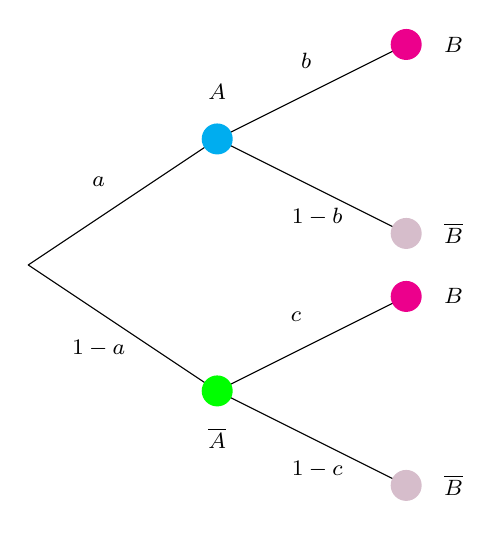
\begin{tikzpicture}[scale=0.8, font=\footnotesize, line join=round, line cap=round, >=stealth]
	\draw (0,0)--(3,2) node [midway, shift=(140:4mm)] {$a$} --(6,3.5) node [midway, shift=(100:4mm)] {$b$};
	\draw (0,0)--(3,-2) node [midway, shift=(-140:4mm)] {$1-a$} --(6,-3.5) node [midway, shift=(-80:4mm)] {$1-c$};
	\draw (3,2)--(6,0.5) node [midway, shift=(-80:4mm)] {$1-b$};
	\draw (3,-2)--(6,-0.5) node [midway, shift=(120:4mm)] {$c$};
	\draw[draw=none,fill=cyan] (3,2) circle [radius=7pt] node[shift=(90:6mm)] {$A$};
	\draw[draw=none,fill=green] (3,-2) circle [radius=7pt] node[shift=(-90:6mm)] {$\overline{A}$};
	\draw[draw=none,fill=magenta] (6,3.5) circle [radius=7pt] node[shift=(0:6mm)] {$B$};
	\draw[draw=none,fill=magenta!40!black!30] (6,0.5) circle [radius=7pt] node[shift=(0:6mm)] {$\overline{B}$};
	\draw[draw=none,fill=magenta] (6,-0.5) circle [radius=7pt] node[shift=(0:6mm)] {$B$};
	\draw[draw=none,fill=magenta!40!black!30] (6,-3.5) circle [radius=7pt] node[shift=(0:6mm)] {$\overline{B}$};
\end{tikzpicture}}
\end{dang}
\boxmini{BÀI TẬP TỰ LUẬN}
\setcounter{vd}{0}
\begin{vd}%[CD]%[Lê Vũ Hải, BG12-4in1]%[2D5N2-3] 
	Cho hai biến cố $A$, $B$ sao cho $\mathrm{P}(A) = 0{,}6$; $\mathrm{P}(B)=0{,}4$; $\mathrm{P}(A|B) = 0{,}3$. Tính $\mathrm{P}(B|A)$.
	\loigiai{
		Áp dụng công thức Bayes, ta có
		\[\mathrm{P}(B|A)=\dfrac{\mathrm{P}(B)\cdot \mathrm{P}(A|B)}{\mathrm{P}(A)}=\dfrac{0{,}4\cdot 0{,}3}{0{,}6}=0{,}2.\]
	}
\end{vd}
\dongcham{3}
\begin{vd}%[CKP]%[Lê Vũ Hải, BG12-4in1]%[2D5H2-3] 
	Kết quả khảo sát tại một xã cho thấy có $20 \%$ cư dân hút thuốc lá. Tỉ lệ cư dân thường xuyên gặp các vấn đề sức khoẻ về đường hô hấp trong số những người hút thuốc lá và không hút thuốc lá lần lượt là $70\%$, $15\%$. Giả sử ta gặp một cư dân của xã, gọi $A$ là biến cố \lq\lq Người đó có hút thuốc lá\rq\rq\, và $B$ là biến cố \lq\lq Người đó thường xuyên gặp các vấn đề sức khoẻ về đường hô hấp\rq\rq.
	\begin{enumerate}
		\item Vẽ sơ đồ hình cây.
		\item Nếu ta gặp một cư dân của xã thì xác suất người đó thường xuyên gặp các vấn đề sức khoẻ về đường hô hấp là bao nhiêu?
		\item  Nếu ta gặp một cư dân của xã thường xuyên gặp các vấn đề sức khoẻ về đường hô hấp thì xác suất người đó có hút thuốc lá là bao nhiêu?
	\end{enumerate}
	\loigiai{
		\begin{enumerate}
			\item Ta có sơ đồ hình cây sau.
			\begin{center}
				\begin{tikzpicture}[scale=.3,>=stealth,every node/.style={shape=rectangle,draw,rounded corners, color=blue, fill=blue!10}]
					%-------------
					\tikzstyle{block} = [rectangle, draw, fill=blue!10, rounded corners, text centered, text width = 10em, minimum height = 2em]
					%-------------
					\node (c1) {Gặp một cư dân};
					\node (c2) [above right = 2cm of c1]{$A$};
					\node (c3) [ below right= 2cm of c1]{$\overline{A}$};
					\node (c4) [above right = 1cm of c2]{$B$} ;
					\node (c5) [below right = 1cm of c2]{$\overline{B}$};
					\node (c6) [ above right =1cm of c3]{$B$};
					\node (c7) [ below right = 1cm of c3]{$\overline{B}$};
					%--------------
					\draw 
					(17.5,15) node[right] {\text{Kết quả}} 
					(20,11.3) node[right] {$AB$} 
					(20,2.5) node[right] {$A\overline{B}$} 
					(20,-2.5) node[right] {$\overline{A}B$} 
					(20,-11.5) node[right] {$\overline{A} \,\,\overline{B}$};
					%--------------
					\draw 
					(25,15) node[right] {\text{Xác suất}} 
					(25,11.3) node[right] {$0{,}14$} 
					(25,2.5) node[right] {$0{,}06$} 
					(25,-2.5) node[right] {$0{,}12$} 
					(25,-11.5) node[right] {$0{,}68$};
					%------------
					\draw[->] (c1.east) --node[above left]{$0{,}2$} (c2.west);
					\draw[->] (c1.east) --node[below left]{$0{,}8$} (c3.west);
					\draw[->] (c2.east) --node[above left]{$0{,}7$} (c4.west);
					\draw[->] (c2.east) --node[below left]{$0{,}3$} (c5.west);
					\draw[->] (c3.east) --node[above left]{$0{,}15$} (c6.west);
					\draw[->] (c3.east) -- node[below left]{$0{,}85$} (c7.west);
				\end{tikzpicture}
			\end{center}
			\item Ta có $\mathrm{P}(B)=\mathrm{P}(A) \cdot \mathrm{P}(B | A)+\mathrm{P}(\overline{A}) \cdot \mathrm{P}\left(B | \overline{A}\right)=0{,}14+0{,}12=0{,}26$.\\
			Vậy nếu ta gặp một cư dân của xã thì xác suất người đó thường xuyên gặp các vấn đề sức khoẻ về đường hô hấp là $26\%$.
			\item Theo công thức Bayes, ta có $\mathrm{P}\left(A | B\right)=\dfrac{\mathrm{P}(A)\cdot \mathrm{P}\left(B| A\right)}{\mathrm{P}(B)}=\dfrac{0{,}14}{0{,}26} \approx 0{,}54$.\\
			Vậy nếu ta gặp một cư dân của xã thường xuyên gặp các vấn đề sức khoẻ về đường hô hấp thì xác suất người đó có hút thuốc lá là khoảng $54\%$.
		\end{enumerate}
	}
\end{vd}
\dongcham{12}
\begin{vd}%[CD]%[Lê Vũ Hải, BG12-4in1]%[2D5H2-3] 
	Giả sử có một loại bệnh mà tỉ lệ người mắc bệnh là $0{,}1\%$. Giả sử có một loại xét nghiệm, mà ai mắc bệnh khi xét nghiệm cũng có phản ứng dương tính, nhưng tỉ lệ phản ứng dương tính giả là $5\%$ (tức là trong số những người không bị bệnh có $5\%$ số người xét nghiệm lại có phản ứng dương tính).
	\begin{enumerate}
		\item Vẽ sơ đồ cây biểu thị tình huống trên.
		\item Khi một người xét nghiệm có phản ứng dương tính thì khả năng mắc bệnh của người đó là bao nhiêu phần trăm (làm tròn kết quả đến hàng phần trăm).
	\end{enumerate}
	\loigiai{
		\begin{enumerate}
			\item Xét hai biến cố
			\begin{itemize}
				\item[] $K$: \lq\lq Người được chọn ra không mắc bệnh\rq\rq.
				\item[] $D$: \lq\lq Người được chọn ra có phản ứng dương tính\rq\rq. 
			\end{itemize}
			Do tỉ lệ người mắc bệnh là là $0,1\%=0{,}001$ nên $\mathrm{P}(K)=1-0{,}001 = 0{,}999$.\\
			Trong số những người không mắc bệnh có $5\%$ số người có phản ứng dương tính nên \break $\mathrm{P}(D|K) = 5\% = 0{,}05$. Vì ai mắc bệnh khi xét nghiệm cũng có phản ứng dương tính nên $\mathrm{P}\left(\overline{K}\right)=1$.\\
			Ta có sơ đồ cây biểu thị tình huống đã cho
			\begin{center}
				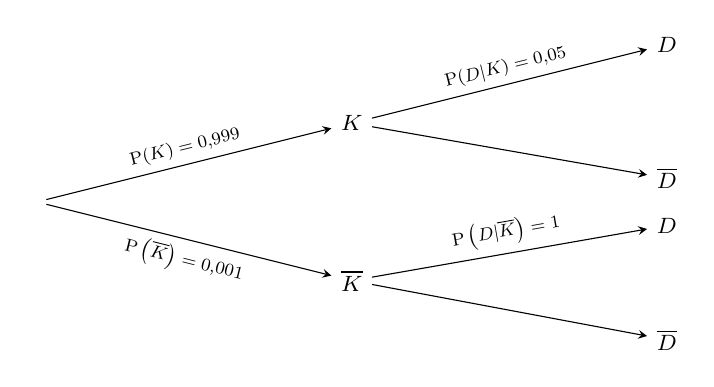
\begin{tikzpicture}[->,>=stealth,line join=round,line cap=round,font=\footnotesize,scale=1]
					\def\xmot{4}
					\def\xhai{8}
					\node (O) at (0,0){};
					\node (B) at (\xmot,1){$K$};
					\node (B1) at (\xmot,-1){$\overline{K}$};
					\node (BA) at (\xhai,2){$D$};
					\node (BA1) at (\xhai,0.3){$\overline{D}$};
					\node (B1A) at (\xhai,-0.3){$D$};
					\node (B1A1) at (\xhai,-1.75){$\overline{D}$};
					
					\foreach \x/\y/\p/\l in 
					{
						O/B/above/$\mathrm{P}(K)=0{,}999$,
						B/BA/above/$\mathrm{P}(D|K)=0{,}05$,
						B/BA1//,
						O/B1/below/$\mathrm{P}\left(\overline{K}\right)=0{,}001$,
						B1/B1A/above/$\mathrm{P}\left(D|\overline{K}\right)=1$,
						B1/B1A1//
					}
					{
						\draw[->] (\x)--(\y)node[midway,\p,scale=0.8,sloped]{\l};
					}
				\end{tikzpicture}
			\end{center}
			\item Ta thấy rằng khả năng mắc bệnh của một người xét nghiệm có phản ứng dương tính chính là $\mathrm{P}\left(\overline{K}|D\right)$. Áp dụng công thức Bayes, ta có:
			\[\mathrm{P}\left(\overline{K}|D\right)=\dfrac{\mathrm{P}\left(\overline{K}\right)\cdot \mathrm{P}\left(D|\overline{K}\right)}{\mathrm{P}\left(\overline{K}\right)\cdot \mathrm{P}\left(D|\overline{K}\right) + \mathrm{P}(K)\cdot\mathrm{P}(D|K)}=\dfrac{0{,}001\cdot 1}{0{,}001\cdot 1 + 0{,}999 \cdot 0{,}05}\approx 1{,}96\%.\]
			Vậy xác suất mắc bệnh của một người xét nghiệm có phản ứng dương tính là $1{,}96\%$.
		\end{enumerate}
	}
\end{vd}
\dongcham{12}
\begin{vd}
	Một nhà máy có hai phân xưởng I và II. Phân xưởng I sản xuất $40\%$ số sản phẩm 
	và phân xưởng II sản xuất $60\%$ số sản phẩm. Tỉ lệ sản phẩm bị lỗi của phần xưởng I 
	là $2\%$ và của phân xưởng II là $1\%$.
	\begin{listEX}
		\item  Kiểm tra ngẫu nhiên 1 sản phẩm của nhà máy và tính xác suất để sản phẩm đó bị lỗi. 
		\item Biết rằng sản phẩm được chọn bị lỗi. Hỏi xác suất sản phẩm đó do phân xưởng nào
		sản xuất cao hơn?
	\end{listEX}
	\loigiai{\begin{listEX}
			\item  Gọi $A$ là biến cố “Sản phẩm bị lỗi” và $B$ là biến cố “Sản phẩm lấy ra do phân xưởng I 
			sản xuất”.\\
			Do phân xưởng I sản xuất $40\%$ số sản phẩm và phân xưởng II sản xuất $60\%$ số sản phẩm nên
			$$\mathrm{P}(B)=0{,}4 \text{ và } \mathrm{P}(\overline{B})=1-0{,}4=0{,}6.$$
			Do tỉ lệ sản phẩm bị lỗi của phân xưởng I là $2\%$ và của phân xưởng II là $1\%$ nên
			$$\mathrm{P}(A|B)=0{,}02 \text{ và } \mathrm{P}(A|\overline{B})=0{,}01.$$
			Xác suất để sản phẩm lấy ra bị lỗi là
			$$\mathrm{P}(A)=\mathrm{P}(B)\mathrm{P}(A|B)+\mathrm{P}(\overline{B})\mathrm{P}(A|\overline{B})=0{,}4\cdot0{,}02+0{,}6 \cdot 0{,}01=0{,}014.$$
			\item Nếu sản phẩm lấy ra bị lỗi thì xác suất sản phẩm đó do phân xưởng I sản xuất là 
			$$\mathrm{P}(B|A)=\dfrac{\mathrm{P}(B)\mathrm{P}(A|B)}{\mathrm{P}(A)}=\dfrac{0{,}4 \cdot 0{,}02}{0{,}014}=\dfrac{4}{7}.$$
			Nếu sản phẩm lấy ra bị lỗi thì xác suất sản phẩm đó do phân xưởng II sản xuất là 
			$$\mathrm{P}(\overline{B}|A)=1-\mathrm{P}(B|A)=\dfrac{3}{7}.$$
			Vậy nếu sản phẩm lấy ra bị lỗi thì xác suất sản phẩm đó do phân xưởng I sản xuất cao hơn 
			xác suất sản phẩm đó do phân xưởng II sản xuất.
	\end{listEX}}
\end{vd}
\dongcham{13}

\begin{vd}
	%	\immini{
		Một loại xét nghiệm nhanh SARS-CoV-2 cho
		kết quả dương tính với $76,2\%$ các ca thực sự
		nhiễm virus và kết quả âm tính với $99,1\%$ các
		ca thực sự không nhiễm virus (nguồn: https://
		tapchiyhocvietnam.vn/index.php/vmj/article/
		view/2124/1921). Giả sử tỉ lệ người nhiễm virus
		SARS-CoV-2 trong một cộng đồng là $1\%$.
		%	}{\includegraphics[scale=0.5]{images/12-SGK-CTST-6-2-1.png}}
	Một người làm xét nghiệm và nhận được kết quả dương tính.
	Tính xác suất người đó thực sự nhiễm virus (kết quả làm tròn đến hàng phần nghìn).
	\loigiai{
		Gọi $A$ là biến cố “Người làm xét nghiệm có kết quả dương tính” và $B$ là biến cố
		“Người làm xét nghiệm thực sự nhiễm virus”.\\
		Do xét nghiệm cho kết quả dương tính với $76,2\%$ các ca thực sự nhiễm virus nên $\mathrm{P}(A|B)=0{,}762$.\\
		Do xét nghiệm cho kết quả âm tính với $99,1\%$ các ca thực sự không nhiễm virus nên
		$\mathrm{P}(\overline{A}|\overline{B})=0{,}991$. Suy ra $$\mathrm{P}(A|\overline{B})=1-0{,}991=0{,}009.$$
		Do tỉ lệ người nhiễm virus trong cộng đồng là $1\%$ nên $\mathrm{P}(B)=0,01$ và $\mathrm{P}(\overline{B}) = 0,99$.
		Áp dụng công thức xác suất toàn phần, ta có xác suất người làm xét nghiệm có kết quả
		dương tính là $$\mathrm{P}(A)=\mathrm{P}(B)\mathrm{P}(A|B)+\mathrm{P}(\overline{B})\mathrm{P}(A|\overline{B})=0{,}01\cdot0{,}762+0{,}99\cdot0{,}009=0{,}01653.$$
		Xác suất một người thực sự nhiễm virus khi người đó có kết quả xét nghiệm dương tính 
		là $\mathrm{P}(B|A)$. Ta có $$\mathrm{P}(B|A)=\dfrac{\mathrm{P}(B)\mathrm{P}(A|B)}{\mathrm{P}(A)}=\dfrac{0{,}01\cdot0{,}762}{0{,}01653}\approx0{,}461.$$}
\end{vd}
\dongcham{14}


\begin{vd}
	Có hai chuồng thỏ. Chuồng thứ nhất có $5$ thỏ đen và $10$ thỏ trắng. Chuồng thứ hai có $7$ thỏ đen và $3$ thỏ trắng. Từ chuồng thứ hai, bắt ngẫu nhiên $1$ con thỏ cho vào chuồng thứ nhất. Sau đó bắt ngẫu nhiên một con thỏ ở chuồng thứ nhất ra thì thấy con thỏ này là thỏ trắng. Tính xác suất để con thỏ bắt ra này thuộc chuồng thứ nhất.
	\loigiai{
		Gọi $E_1$ là biến cố: ``Bắt được thỏ trắng ở lần thứ nhất'', dễ thấy $P(E_1) = \dfrac{3}{10} = 0,3$.\\
		Gọi $E_2$ là biến cố: ``Bắt được thỏ đen ở lần thứ nhất'', dễ thấy $P(E_2) = \dfrac{7}{10} = 0,7$.\\
		Gọi $A$ là biến cố: ``Bắt được thỏ trắng ở lần thứ hai'' và $B$ là biến cố: ``Con thỏ bắt được ở lần thứ hai là thỏ gốc của chuồng thứ nhất''.\\
		Nhận xét: Ở lần bắt thỏ đầu tiên, nếu bắt được thỏ trắng ở chuồng thứ hai thì chuồng thứ nhất có $5$ thỏ đen, $11$ thỏ trắng; nếu bắt được thỏ đen ở chuồng thứ hai thì chuồng thứ nhất có $6$ thỏ đen và $10$ thỏ trắng.\\
		Xác suất để con thỏ bắt ra ở lần thứ hai là thỏ trắng:
		$$P(A) = P(E_1)P(A|E_1) + P(E_2)P(A|E_2) = \dfrac{3}{10} \cdot \dfrac{11}{16} + \dfrac{7}{10} \cdot \dfrac{10}{16} = \dfrac{103}{160}.$$
		Xác suất để con thỏ bắt ra ở lần thứ hai là thỏ trắng và thuộc chuồng 1 (tức là chọn trúng $1$ trong $10$ con thỏ trắng ban đầu của chuồng 1, điều này luôn xảy ra với xác suất $\dfrac{10}{16}$ dù thỏ chuyển sang là màu gì):
		$$P(AB) = P(E_1)P(AB|E_1) + P(E_2)P(AB|E_2) = \dfrac{3}{10} \cdot \dfrac{10}{16} + \dfrac{7}{10} \cdot \dfrac{10}{16} = \dfrac{10}{16} = \dfrac{100}{160}.$$
		Xác suất cần tìm (xác suất có điều kiện):
		$$P(B|A) = \dfrac{P(AB)}{P(A)} = \dfrac{\dfrac{100}{160}}{\dfrac{103}{160}} = \dfrac{100}{103}.$$
	}
\end{vd}

\dongcham{18}
\boxmini{BÀI TẬP TRẮC NGHIỆM}
\setcounter{ex}{0}
\Opensolutionfile{ans}[ans/2D6-B2-d2-1]
\begin{ex}%[Mức độ 1]%[Lê Vũ Hải, BG12-4in1]%[2D5N2-3] 
	Cho $\mathrm{P}(A)=\dfrac{2}{5}$; $\mathrm{P}\left( B\mid A\right)=\dfrac{1}{3}$; $\mathrm{P}\left(B\mid \overline{A}\right)=\dfrac{1}{4}$. Giá trị của $\mathrm{P}(A\mid B)$ là 
	\choice
	{$\dfrac{7}{17} $}
	{\True $ \dfrac{8}{17}$}
	{$ \dfrac{5}{17}$}
	{$ \dfrac{9}{17}$}
	\loigiai{Áp dụng công thức Bayes ta có
		$$\mathrm{P}(A\mid B)=\dfrac{\mathrm{P}(A)\cdot \mathrm{P}(B\mid A)}{\mathrm{P}(A)\cdot \mathrm{P}(B\mid A)+\mathrm{P}\left( \overline{A}\right) \cdot \mathrm{P}\left( B\mid \overline{A}\right) }=\dfrac{\dfrac{2}{5}\cdot \dfrac{1}{3}}{\dfrac{2}{5}\cdot \dfrac{1}{3}+\dfrac{3}{5}\cdot \dfrac{1}{4}}=\dfrac{8}{17}.$$
	}
\end{ex}\cham{5}

\begin{ex}%[Mức độ 2]%[Lê Vũ Hải, BG12-4in1]%[2D5H2-3] 
	Cho $\mathrm{P}(A)=\dfrac{4}{5}$; $\mathrm{P}\left( B\mid A\right)=\dfrac{2}{3}$; $\mathrm{P}\left(B\mid \overline{A}\right)=\dfrac{1}{4}$. Giá trị của $\mathrm{P}(A\mid B)$ là 
	\choice
	{$\dfrac{33}{35} $}
	{\True $ \dfrac{32}{35}$}
	{$ \dfrac{9}{35}$}
	{$ \dfrac{26}{35}$}
	\loigiai{Áp dụng công thức Bayes ta có
		$$\mathrm{P}(A\mid B)=\dfrac{\mathrm{P}(A)\cdot \mathrm{P}(B\mid A)}{\mathrm{P}(A)\cdot \mathrm{P}(B\mid A)+\mathrm{P}\left( \overline{A}\right) \cdot \mathrm{P}\left( B\mid \overline{A}\right) }=\dfrac{\dfrac{4}{5}\cdot \dfrac{2}{3}}{\dfrac{4}{5}\cdot \dfrac{2}{3}+\dfrac{1}{5}\cdot \dfrac{1}{4}}=\dfrac{32}{35}.$$
	}
\end{ex}\cham{5}



%Bt 6.18
\begin{ex}%[Mức độ 2]%[Lê Vũ Hải, BG12-4in1]%[2D5H2-3] 
	Cho $A$, $B$ là các biến cố thỏa mãn $\mathrm{P}(\overline{A}\,. \overline{B})=0{,}35$, $\mathrm{P}(A)=0{,}25$, $\mathrm{P}(B)=0{,}6$. Giá trị của $\mathrm{P}(A|B)$ bằng
	\choice
	{$\dfrac{1}{5}$}
	{\True$\dfrac{1}{3}$}
	{$\dfrac{7}{15}$}
	{$\dfrac{2}{3}$}
	\loigiai{
		Ta có $\mathrm{P}\left( {\overline {A} \,.\overline{B} } \right) = \mathrm{P}\left( {\overline A } \right)\mathrm{P}\left( {\overline B |\overline A } \right) \Rightarrow \mathrm{P}\left( {\overline B |\overline A } \right) = \dfrac{{\mathrm{P}\left( {\overline {A}\,.\overline{B} } \right)}}{{\mathrm{P}\left( {\overline A } \right)}} = \dfrac{{0{,}35}}{{0{,}75}} = \dfrac{7}{{15}}.$ \\
		Suy ra $\mathrm{P}\left( {B|\overline A } \right) = 1 - \dfrac{7}{{15}} = \dfrac{8}{{15}}$.\\
		Theo công thức xác suất toàn phần, ta có
		$$\begin{array}{l}
			\mathrm{P}\left( B \right) = \mathrm{P}\left( {B|A} \right) \mathrm{P}\left( A \right) + \mathrm{P}\left( {B|\overline A } \right) \mathrm{P}\left( {\overline A } \right)\\
			\Rightarrow \mathrm{P}\left( {B|A} \right) = \dfrac{{\mathrm{P}\left( B \right) - \mathrm{P}\left( {B|\overline A } \right) \mathrm{P}\left( {\overline A } \right)}}{{\mathrm{P}\left( A \right)}} = \dfrac{{0{,}6 - \dfrac{8}{{15}} \cdot 0{,}75}}{{0{,}25}} = 0{,}8.
		\end{array}$$
		Theo công thức Bayes, ta được
		$$\mathrm{P}\left( {A|B} \right) = \dfrac{{\mathrm{P}\left( A \right) \mathrm{P}\left( {B|A} \right)}}{{\mathrm{P}\left( B \right)}} = \dfrac{{0{,}25 \cdot 0{,}8}}{{0{,}6}} = \dfrac{1}{3}.$$}
\end{ex}\cham{5}

\begin{ex}%[Mức độ 2]%[Lê Vũ Hải, BG12-4in1]%[2D5H2-3] 
	\immini[thm]{Cho sơ đồ hình cây như hình bên. Biết $\mathrm{P}(A)=0{,}6$. Tính $\mathrm{P}(A \mid B)$.
		\choice
		{$\dfrac{6}{11}$}
		{$\dfrac{7}{11}$}
		{$\dfrac{8}{11}$}
		{\True $\dfrac{9}{11}$}}		
	{
	
		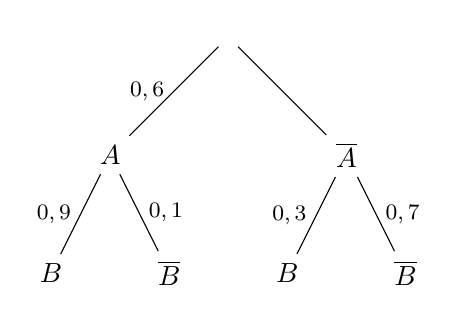
\begin{tikzpicture}[level 1/.style={sibling distance=3cm}, level 2/.style={sibling distance=1.5cm}]
			\node {}
			child {node {$A$}
				child {node {$B$} edge from parent node[left, font=\footnotesize] {$0,9$}}
				child {node {$\overline{B}$} edge from parent node[right, font=\footnotesize] {$0,1$}}
				edge from parent node[left, font=\footnotesize] {$0,6$}
			}
			child {node {$\overline{A}$}
				child {node {$B$} edge from parent node[left, font=\footnotesize] {$0,3$}}
				child {node {$\overline{B}$} edge from parent node[right, font=\footnotesize] {$0,7$}}
				edge from parent node[right, font=\footnotesize] {}
			};
	\end{tikzpicture}}
	\loigiai{
		Theo công thức Bayes ta có \begin{eqnarray*}
			\mathrm{P}\left( {A|B} \right) &=& \dfrac{{\mathrm{P}\left( A \right) \mathrm{P}\left( {B|A} \right)}}{{P\left( B \right)}} \\
			&=& \dfrac{{\mathrm{P}\left( A \right)\mathrm{P}\left( {B|A} \right)}}{\mathrm{P}(A) \cdot \mathrm{P}(B \mid A)+\mathrm{P}(\overline{A}) \cdot \mathrm{P}(B \mid \overline{A})} \\
			&=& \dfrac{0{,}6 \cdot 0{,}9}{0{,}6 \cdot 0{,}9+0{,}4 \cdot 0{,}3} = \dfrac{9}{11}.
		\end{eqnarray*}
	}
\end{ex}\cham{1}

\begin{ex}%[Mức độ 2]%[Lê Vũ Hải, BG12-4in1]%[2D5H2-3] 
	\immini[thm]{Cho sơ đồ hình cây như hình bên. Biết $\mathrm{P}(A)=0{,}48$. Tính $\mathrm{P}(A \mid B)$ là
		\choice
		{$\dfrac{26}{49}$}
		{\True $\dfrac{36}{49}$}
		{$\dfrac{15}{39}$}
		{$\dfrac{36}{59}$}}
	{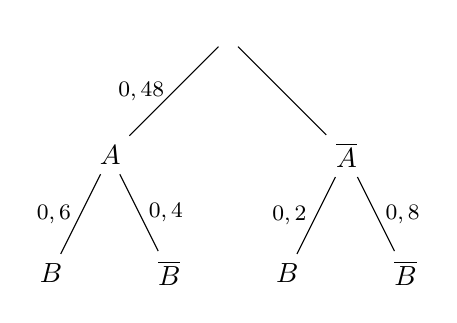
\begin{tikzpicture}[level 1/.style={sibling distance=3cm}, level 2/.style={sibling distance=1.5cm}]
			\node {}
			child {node {$A$}
				child {node {$B$} edge from parent node[left, font=\footnotesize] {$0,6$}}
				child {node {$\overline{B}$} edge from parent node[right, font=\footnotesize] {$0,4$}}
				edge from parent node[left, font=\footnotesize] {$0,48$}
			}
			child {node {$\overline{A}$}
				child {node {$B$} edge from parent node[left, font=\footnotesize] {$0,2$}}
				child {node {$\overline{B}$} edge from parent node[right, font=\footnotesize] {$0,8$}}
				edge from parent node[right, font=\footnotesize] {}
			};
	\end{tikzpicture}}
	\loigiai{
		Theo công thức Bayes ta có \begin{eqnarray*}
			\mathrm{P}\left( {A|B} \right) &=& \dfrac{{\mathrm{P}\left( A \right)\mathrm{P}\left( {B|A} \right)}}{{\mathrm{P}\left( B \right)}} \\
			&=& \dfrac{{\mathrm{P}\left( A \right) \mathrm{P}\left( {B|A} \right)}}{\mathrm{P}(A) \cdot \mathrm{P}(B \mid A)+\mathrm{P}(\overline{A}) \cdot \mathrm{P}(B \mid \overline{A})} \\
			&=& \dfrac{0{,}48 \cdot 0{,}6}{0{,}48 \cdot 0{,}6+0{,}52 \cdot 0{,}2} = \dfrac{36}{49}.
		\end{eqnarray*}
	}
\end{ex}
\cham{1}
\begin{ex}%[Mức độ 2]%[Lê Vũ Hải, BG12-4in1]%[2D5H2-3] 
	\immini[thm]{Cho sơ đồ hình cây như hình bên. Biết $\mathrm{P}(A)=0{,}72$. Tính $\mathrm{P}(A \mid \overline{B})$ là
		\choice
		{\True $\dfrac{9}{16}$}
		{$\dfrac{16}{25}$}
		{$\dfrac{9}{25}$}
		{$\dfrac{3}{16}$}}
	{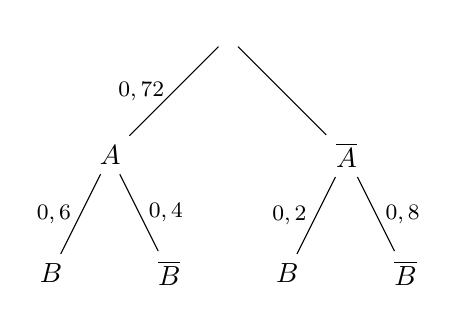
\begin{tikzpicture}[level 1/.style={sibling distance=3cm}, level 2/.style={sibling distance=1.5cm}]
			\node {}
			child {node {$A$}
				child {node {$B$} edge from parent node[left, font=\footnotesize] {$0,6$}}
				child {node {$\overline{B}$} edge from parent node[right, font=\footnotesize] {$0,4$}}
				edge from parent node[left, font=\footnotesize] {$0,72$}
			}
			child {node {$\overline{A}$}
				child {node {$B$} edge from parent node[left, font=\footnotesize] {$0,2$}}
				child {node {$\overline{B}$} edge from parent node[right, font=\footnotesize] {$0,8$}}
				edge from parent node[right, font=\footnotesize] {}
			};
	\end{tikzpicture}}
	\loigiai{
		Theo công thức Bayes ta có \begin{eqnarray*}
			\mathrm{P}\left( {A|\overline{B}} \right) &=& \dfrac{{\mathrm{P}\left( A \right) \mathrm{P}\left( {\overline{B}|A} \right)}}{{\mathrm{P}\left( \overline{B} \right)}} \\
			&=& \dfrac{{\mathrm{P}\left( A \right) \mathrm{P}\left( {\overline{B}|A} \right)}}{\mathrm{P}(A) \cdot \mathrm{P}(\overline{B}\mid A)+\mathrm{P}(\overline{A}) \cdot \mathrm{P}(\overline{B} \mid \overline{A})} \\
			&=& \dfrac{0{,}72 \cdot 0{,}4}{0{,}72 \cdot 0{,}4+0{,}28 \cdot 0{,}8} = \dfrac{9}{16}.
		\end{eqnarray*}
	}
\end{ex}
\cham{1}
\begin{ex}%[Mức độ 2]%[Lê Vũ Hải, BG12-4in1]%[2D5H2-3] 
	Một bệnh viện có hai phòng khám là phòng A và phòng B với khả năng lựa chọn của bệnh nhân là như nhau. Tỉ lệ bệnh nhân nam có ở phòng A và phòng B lần lượt là $60\%$ và $40\%$. Một người bệnh được chọn ngẫu nhiêu từ hai phòng khám và biết người này là nam, xác suất để người bệnh được chọn đến từ phòng A là
	\choice
	{\True $0{,}6$}
	{$0{,}5$}
	{$0{,}4$}
	{$0{,}3$}
	\loigiai{Một người bệnh được chọn ngẫu nhiên từ hai phòng khám.\\
		Gọi $X$ là biến cố \lq \lq Người đó đến từ phòng khám A\rq \rq \, và $Y$, $\overline{Y}$ lần lượt là biến cố \lq \lq Người đó là nam\rq \rq \; và \lq \lq Người đó không là nam\rq \rq.\\
		Ta có sơ đồ hình cây sau
		\begin{center}
			\begin{tikzpicture}[>=stealth,scale=0.8]
				%Khung 1
				\draw (-3.5,-1) rectangle (2.2,0);
				\draw (-0.8,-0.5) node{Bệnh nhân được chọn} ;
				%Mui ten 1,2
				\draw [->] (2.2,-0.5)--(3.8,1.6) node[pos=0.5,sloped,above]{$0{,}5$};
				\draw [->] (2.2,-0.5)--(3.8,-2.6) node[pos=0.5,sloped,below]{$0{,}5$};
				%Khung 2.1
				\draw (3.8,1.1) rectangle (5.1,2.1);
				\draw (8.9/2,1.6) node{$X$} ;
				%Khung 2.2
				\draw (3.8,-2.1) rectangle (5.1,-3.1);
				\draw (8.9/2,-2.6) node{$\overline{X}$} ;
				%Mui ten 3,4
				\draw [->] (5.1,1.6)--(6.5,2.6) node[pos=0.5,sloped,above]{$0{,}6$};
				\draw [->] (5.1,1.6)--(6.5,0.6) node[pos=0.5,sloped,below]{$0{,}4$};
				%Mui ten 5,6
				\draw [->] (5.1,-2.6)--(6.5,-1.6) node[pos=0.5,sloped,above]{$0{,}4$};
				\draw [->] (5.1,-2.6)--(6.5,-3.6) node[pos=0.5,sloped,below]{$0{,}6$};
				%Khung 3.1
				\draw (6.5,2.2) rectangle (7.7,3.2);
				\draw (7.1,5.4/2) node{$Y$} ;
				%Khung 3.2
				\draw (6.5,1.2) rectangle (7.7,0.2);
				\draw (7.1,1.4/2) node{$\overline{Y}$} ;
				%Khung 3.3
				\draw (6.5,-1.1) rectangle (7.7,-2.1);
				\draw (7.1,-3.2/2) node{$Y$} ;
				%Khung 3.3
				\draw (6.5,-2.9) rectangle (7.7,-3.9);
				\draw (7.1,-3.4) node{$\overline{Y}$} ;
				%Kết quả
				\draw (9.5,3.7) node{\textbf{Kết quả}};	
				\draw (9.5,2.7) node{$XY$};
				\draw (9.5,0.7) node{$X \overline{Y}$};
				\draw (9.5,-1.6) node{$\overline{X}Y$};
				\draw (9.5,-3.4) node{$\overline{X} \,\,\overline{Y}$};
				%Xác suất
				\draw (12.5,3.7) node{\textbf{Xác suất}};	
				\draw (12.5,2.7) node{$0{,}3$};
				\draw (12.5,0.7) node{$0{,}2$};
				\draw (12.5,-1.6) node{$0{,}2$};
				\draw (12.5,-3.4) node{$0{,}3$};	
			\end{tikzpicture}
		\end{center}		
		Theo công thức Bayes, ta có $$\mathrm{P}(X|Y)=\dfrac{\mathrm{P}(X)\mathrm{P}(Y|X)}{\mathrm{P}(X)\mathrm{P}(Y|X)+\mathrm{P}(\overline{X})\mathrm{P}(Y|\overline{X})}=\dfrac{0{,}3}{0{,}3+0{,}2}=0{,}6.$$
		Vậy với một người bệnh được chọn ngẫu nhiêu từ hai phòng khám và biết người này là nam, xác suất để người đó đến từ phòng A là $0{,}6$.}
\end{ex}\cham{5}

\begin{ex}%[Mức độ 3]%[Lê Vũ Hải, BG12-4in1]%[2D5V2-3] 
	Một bệnh viện đang xét nghiệm cho một số bệnh nhân để xác định liệu họ có nhiễm virus $X$ hay không. Xác suất để một bệnh nhân bị nhiễm virus $X$ là $0{,}05$. Khi xét nghiệm, nếu một bệnh nhân bị nhiễm thì xác suất để kết quả xét nghiệm dương tính là $0{,}95$. Nếu một bệnh nhân không bị nhiễm thì xác suất để kết quả xét nghiệm âm tính là $0{,}98$. Một bệnh nhân được chọn ngẫu nhiên và có kết quả xét nghiệm dương tính. Xác suất để bệnh nhân đó thực sự bị nhiễm virus $X$ là
	\choice
	{$\dfrac{133}{2000}$}
	{$\dfrac{19}{400}$}
	{\True $\dfrac{5}{7}$}
	{$\dfrac{2}{7}$}
	\loigiai{Một bệnh nhân đến một bệnh viên để xét nghiệm.\\
		Gọi $A$ là biến cố \lq \lq Bệnh nhân bị nhiễm virus $X$\rq \rq \, và $B$, $\overline{B}$ lần lượt là biến cố \lq \lq Kết quả xét nghiệm dương tính\rq \rq \; và \lq \lq Kết quả xét nghiệm âm tính\rq \rq.\\
		Ta xét sơ đồ hình cây như sau\\
		\begin{tikzpicture}[>=stealth,scale=0.8]
			%Khung 1
			\draw (-4.3,-1) rectangle (2.2,0);
			\draw (-1,-0.5) node{Bệnh nhân được xét nghiệm} ;
			%Mui ten 1,2
			\draw [->] (2.2,-0.5)--(3.8,1.6) node[pos=0.5,sloped,above]{$0{,}05$};
			\draw [->] (2.2,-0.5)--(3.8,-2.6) node[pos=0.5,sloped,below]{$0{,}95$};
			%Khung 2.1
			\draw (3.8,1.1) rectangle (5.1,2.1);
			\draw (8.9/2,1.6) node{$A$} ;
			%Khung 2.2
			\draw (3.8,-2.1) rectangle (5.1,-3.1);
			\draw (8.9/2,-2.6) node{$\overline{A}$} ;
			%Mui ten 3,4
			\draw [->] (5.1,1.6)--(6.5,2.6) node[pos=0.5,sloped,above]{$0{,}95$};
			\draw [->] (5.1,1.6)--(6.5,0.6) node[pos=0.5,sloped,below]{$0{,}05$};
			%Mui ten 5,6
			\draw [->] (5.1,-2.6)--(6.5,-1.6) node[pos=0.5,sloped,above]{$0{,}02$};
			\draw [->] (5.1,-2.6)--(6.5,-3.6) node[pos=0.5,sloped,below]{$0{,}98$};
			%Khung 3.1
			\draw (6.5,2.2) rectangle (7.7,3.2);
			\draw (7.1,5.4/2) node{$B$} ;
			%Khung 3.2
			\draw (6.5,1.2) rectangle (7.7,0.2);
			\draw (7.1,1.4/2) node{$\overline{B}$} ;
			%Khung 3.3
			\draw (6.5,-1.1) rectangle (7.7,-2.1);
			\draw (7.1,-3.2/2) node{$B$} ;
			%Khung 3.3
			\draw (6.5,-2.9) rectangle (7.7,-3.9);
			\draw (7.1,-3.4) node{$\overline{B}$} ;
			%Kết quả
			\draw (9.5,3.7) node{\textbf{Kết quả}};	
			\draw (9.5,2.7) node{$AB$};
			\draw (9.5,0.7) node{$A\overline{B}$};
			\draw (9.5,-1.6) node{$\overline{A}B$};
			\draw (9.5,-3.4) node{$\overline{A}\,.\overline{B}$};
			%Xác suất
			\draw (12.5,3.7) node{\textbf{Xác suất}};	
			\draw (12.5,2.7) node{$0{,}0475$};
			\draw (12.5,0.7) node{$0{,}0025$};
			\draw (12.5,-1.6) node{$0{,}019$};
			\draw (12.5,-3.4) node{$0{,}931$};
		\end{tikzpicture}
		
		Theo công thức Bayes, ta có $$\mathrm{P}(A|B)=\dfrac{\mathrm{P}(A) \mathrm{P}(B|A)}{\mathrm{P}(A) \mathrm{P}(B|A)+\mathrm{P}(\overline{A})\mathrm{P}(B|\overline{A})}=\dfrac{0{,}0475}{0{,}0475+0{,}019}=\dfrac{5}{7}.$$		 
		Vậy với một bệnh nhân có kết quả xét nghiệm dương tính, xác suất để bệnh nhân đó thực sự bị nhiễm virus $X$ là $\dfrac{5}{7}$.}
\end{ex}\cham{5}
%Bt 6.20
\begin{ex}%[Mức độ 3]%[Lê Vũ Hải, BG12-4in1]%[2D5V2-3] 
	Ở một địa phương $X$, xác suất để một người lớn trên $40$ tuổi mắc bệnh ung thư là $0{,}05$. Xác suất bác sĩ chẩn đoán đúng một người mắc bệnh ung thư là $0{,}78$ và chẩn đoán sai (không bị ung thư nhưng được chẩn đoán mắc bệnh) là $0{,}06$. Xác suất để một người thật sự mắc bệnh ung thư khi nhận được kết quả chẩn đoán bị ung thư bằng
	\choice
	{\True$0{,}40625$}
	{$0{,}096$}
	{$0{,}904$}
	{$0{,}59375$}
	\loigiai{Một bệnh nhân trên 40 tuổi ở địa phương X đến bác sĩ để khám bệnh ung thư.\\
		Gọi $A$ là biến cố \lq \lq Người đó mắc bệnh ung thư\rq \rq \, và $B$, $\overline{B}$ lần lượt là biến cố \lq \lq Bác sĩ chẩn đoán người đó bị ung thư\rq \rq \;và \lq \lq Bác sĩ chẩn đoán người đó không bị ung thư\rq \rq.\\
		Ta xét sơ đồ hình cây như sau\\
		\begin{tikzpicture}[>=stealth,scale=0.8]
			%Khung 1
			\draw (-4.3,-1) rectangle (2.2,0);
			\draw (-1,-0.5) node{Bệnh nhân được chẩn đoán} ;
			%Mui ten 1,2
			\draw [->] (2.2,-0.5)--(3.8,1.6) node[pos=0.5,sloped,above]{$0{,}05$};
			\draw [->] (2.2,-0.5)--(3.8,-2.6) node[pos=0.5,sloped,below]{$0{,}95$};
			%Khung 2.1
			\draw (3.8,1.1) rectangle (5.1,2.1);
			\draw (8.9/2,1.6) node{$A$} ;
			%Khung 2.2
			\draw (3.8,-2.1) rectangle (5.1,-3.1);
			\draw (8.9/2,-2.6) node{$\overline{A}$} ;
			%Mui ten 3,4
			\draw [->] (5.1,1.6)--(6.5,2.6) node[pos=0.5,sloped,above]{$0{,}78$};
			\draw [->] (5.1,1.6)--(6.5,0.6) node[pos=0.5,sloped,below]{$0{,}22$};
			%Mui ten 5,6
			\draw [->] (5.1,-2.6)--(6.5,-1.6) node[pos=0.5,sloped,above]{$0{,}06$};
			\draw [->] (5.1,-2.6)--(6.5,-3.6) node[pos=0.5,sloped,below]{$0{,}94$};
			%Khung 3.1
			\draw (6.5,2.2) rectangle (7.7,3.2);
			\draw (7.1,5.4/2) node{$B$} ;
			%Khung 3.2
			\draw (6.5,1.2) rectangle (7.7,0.2);
			\draw (7.1,1.4/2) node{$\overline{B}$} ;
			%Khung 3.3
			\draw (6.5,-1.1) rectangle (7.7,-2.1);
			\draw (7.1,-3.2/2) node{$B$} ;
			%Khung 3.3
			\draw (6.5,-2.9) rectangle (7.7,-3.9);
			\draw (7.1,-3.4) node{$\overline{B}$} ;
			%Kết quả
			\draw (9.5,3.7) node{\textbf{Kết quả}};	
			\draw (9.5,2.7) node{$AB$};
			\draw (9.5,0.7) node{$A\overline{B}$};
			\draw (9.5,-1.6) node{$\overline{A}B$};
			\draw (9.5,-3.4) node{$\overline{A}\,.\overline{B}$};
			%Xác suất
			\draw (12.5,3.7) node{\textbf{Xác suất}};	
			\draw (12.5,2.7) node{$0{,}039$};
			\draw (12.5,0.7) node{$0{,}011$};
			\draw (12.5,-1.6) node{$0{,}057$};
			\draw (12.5,-3.4) node{$0{,}893$};
		\end{tikzpicture}
		
		Theo công thức Bayes, ta có $$\mathrm{P}(A|B)=\dfrac{\mathrm{P}(A) \mathrm{P}(B|A)}{\mathrm{P}(A) \mathrm{P}(B|A)+\mathrm{P}(\overline{A}) \mathrm{P}(B|\overline{A})}=\dfrac{0{,}039}{0{,}039+0{,}057}=0{,}40625.$$		 
		Vậy xác suất để một người thật sự mắc bệnh ung thư khi nhận được kết quả chẩn đoán bị ung thư bằng $0{,}40625$.}
\end{ex}\cham{5} 

\begin{ex}%[Mức độ 4]
	Một hộp có $3$ bi trắng và $4$ bi đen. Hộp thứ hai có $4$ bi trắng và $5$ bi đen. Rút ngẫu nhiên một viên bi từ hộp thứ nhất bỏ vào hộp thứ hai, sau đó rút ngẫu nhiên một viên bi từ hộp thứ hai ra. Biết rằng viên bi lấy ra từ hộp thứ hai là bi trắng. Tính xác suất để viên bi chuyển từ hộp thứ nhất sang là bi đen.
	\choice
	{$\dfrac{4}{7}$}
	{$\dfrac{12}{31}$}
	{\True $\dfrac{16}{31}$}
	{$\dfrac{15}{31}$}
	\loigiai{
		Gọi $A_1$ là biến cố ``Viên bi chuyển từ hộp 1 sang là bi trắng'', $P(A_1) = \dfrac{3}{7}$.
		Gọi $A_2$ là biến cố ``Viên bi chuyển từ hộp 1 sang là bi đen'', $P(A_2) = \dfrac{4}{7}$.
		Hệ $\{A_1, A_2\}$ là một hệ đầy đủ.
		Gọi $B$ là biến cố ``Viên bi lấy ra từ hộp 2 là bi trắng''.\\
		Nếu $A_1$ xảy ra (chuyển bi trắng), hộp 2 sẽ có $5$ trắng và $5$ đen. $P(B|A_1) = \dfrac{5}{10} = \dfrac{1}{2}$.\\
		Nếu $A_2$ xảy ra (chuyển bi đen), hộp 2 sẽ có $4$ trắng và $6$ đen. $P(B|A_2) = \dfrac{4}{10} = \dfrac{2}{5}$.
		Xác suất toàn phần để lấy được bi trắng từ hộp 2:
		$P(B) = P(A_1)P(B|A_1) + P(A_2)P(B|A_2) = \dfrac{3}{7} \cdot \dfrac{1}{2} + \dfrac{4}{7} \cdot \dfrac{2}{5} = \dfrac{3}{14} + \dfrac{8}{35} = \dfrac{31}{70}$.
		Xác suất viên bi chuyển sang là bi đen với điều kiện rút ra từ hộp 2 là bi trắng:
		$P(A_2|B) = \dfrac{P(A_2)P(B|A_2)}{P(B)} = \dfrac{\dfrac{8}{35}}{\dfrac{31}{70}} = \dfrac{16}{31}$.
	}
\end{ex}
\cham{5}
\begin{ex}%[Mức độ 4]
	Một sinh viên làm bài thi trắc nghiệm. Xác suất sinh viên học thuộc bài là $0{,}6$. Nếu thuộc bài, xác suất sinh viên làm đúng là $0{,}9$. Nếu không thuộc bài, sinh viên chọn đáp án ngẫu nhiên với xác suất đúng là $0{,}25$. Biết rằng sinh viên đó đã làm đúng một câu hỏi. Xác suất sinh viên đó KHÔNG thuộc bài là bao nhiêu?
	\choice
	{$\dfrac{5}{14}$}
	{$\dfrac{1}{4}$}
	{\True $\dfrac{5}{32}$}
	{$\dfrac{27}{32}$}
	\loigiai{
		Gọi $A_1$ là biến cố ``Sinh viên thuộc bài'', $P(A_1) = 0{,}6$.
		Gọi $A_2$ là biến cố ``Sinh viên không thuộc bài'', $P(A_2) = 1 - 0{,}6 = 0{,}4$.
		Gọi $D$ là biến cố ``Sinh viên làm đúng câu hỏi''.
		Ta có: $P(D|A_1) = 0{,}9$ và $P(D|A_2) = 0{,}25$.
		Xác suất toàn phần sinh viên làm đúng:
		$P(D) = P(A_1)P(D|A_1) + P(A_2)P(D|A_2) = 0{,}6 \cdot 0{,}9 + 0{,}4 \cdot 0{,}25 = 0{,}54 + 0{,}10 = 0{,}64$.
		Xác suất sinh viên không thuộc bài khi biết đã làm đúng:
		$P(A_2|D) = \dfrac{P(A_2)P(D|A_2)}{P(D)} = \dfrac{0{,}10}{0{,}64} = \dfrac{10}{64} = \dfrac{5}{32}$.
	}
\end{ex}
\cham{4}
\begin{ex}%[Mức độ 3]
	Xác suất để một chuyến bay cất cánh đúng giờ nếu trời không mưa là $0{,}9$. Nếu trời mưa, xác suất chuyến bay cất cánh đúng giờ chỉ còn $0{,}3$. Dự báo thời tiết cho thấy xác suất trời mưa vào ngày mai là $0{,}2$. Biết rằng chuyến bay ngày mai cất cánh CHẬM giờ. Hãy tính xác suất trời đã mưa.
	\choice
	{\True $\dfrac{7}{11}$}
	{$\dfrac{7}{15}$}
	{$\dfrac{2}{5}$}
	{$\dfrac{8}{15}$}
	\loigiai{
		Gọi $M$ là biến cố ``Ngày mai trời mưa'', $P(M) = 0{,}2$. Suy ra $P(\overline{M}) = 0{,}8$.
		Gọi $C$ là biến cố ``Chuyến bay cất cánh chậm giờ'' (tức là không đúng giờ).
		Xác suất chậm giờ nếu không mưa: $P(C|\overline{M}) = 1 - 0{,}9 = 0{,}1$.
		Xác suất chậm giờ nếu trời mưa: $P(C|M) = 1 - 0{,}3 = 0{,}7$.
		Xác suất toàn phần để chuyến bay chậm giờ:
		$P(C) = P(M)P(C|M) + P(\overline{M})P(C|\overline{M}) = 0{,}2 \cdot 0{,}7 + 0{,}8 \cdot 0{,}1 = 0{,}14 + 0{,}08 = 0{,}22$.
		Áp dụng công thức Bayes, xác suất trời mưa khi biết máy bay cất cánh chậm giờ là:
		$P(M|C) = \dfrac{P(M)P(C|M)}{P(C)} = \dfrac{0{,}14}{0{,}22} = \dfrac{7}{11}$.
	}
\end{ex}
\cham{4}
\begin{ex}%Câu 2.3
	Một phần mềm nhận dạng tin nhắn quảng cáo trên điện thoại bằng cách dựa theo từ khóa để đánh dấu một số tin nhắn được gửi đến. Qua một thời gian dài sử dụng, người ta thấy rằng trong số tất cả các tin nhắn gửi đến, có $15 \%$ số tin nhắn bị đánh dấu. Trong số các tin nhắn bị đánh dấu, có $10 \%$ số tin nhắn không phải là quảng cáo. Trong số các tin nhắn không bị đánh dấu, có $5 \%$ số tin nhắn là quảng cáo.
	Chọn ngẫu nhiên một tin nhắn được gửi đến điện thoại. Xét tính đúng sai của các khẳng định sau:
	\choiceTF
	{\True Xác suất để tin nhắn đó không bị đánh dấu bằng $0{,}85$}
	{\True Xác suất để tin nhắn đó không phải là quảng cáo, biết rằng nó không bị đánh dấu, bằng $0{,}95$}
	{Xác suất để tin nhắn đó không phải là quảng cáo bằng $0{,}85$}
	{\True Xác suất để tin nhắn đó không bị đánh dấu, biết rằng nó không phải là quảng cáo, lớn hơn $0{,}95$}
	\loigiai{
		Gọi biến cố $A$ là ``tin nhắn bị đánh dấu'', $B$ là ``tin nhắn quảng cáo'' thì biến cố $\overline{A}$ là ``tin nhắn không bị đánh dấu'' và $\overline{B}$ là ``tin nhắn không quảng cáo''. Ta có sơ đồ hình cây như sau:
		\\
		\centerline{
			\begin{tikzpicture}
				\path
				(0,0) node[rectangle, draw](goc){Tin nhắn}
				(3,2) node[circle, draw](a){$A$}
				(3,-2) node[circle, draw](ax){$\overline{A}$}
				(6,3) node[circle, draw](ab){$B$}
				(6,1) node[circle, draw](abx){$\overline{B}$}
				(6,-1) node[circle, draw](axb){$B$}
				(6,-3) node[circle, draw](axbx){$\overline{B}$}
				;
				\draw[-stealth,thick] (goc)--(a) node[pos=.5,fill=white]{$0{,}15$};
				\draw[-stealth,thick] (goc)--(ax) node[pos=.5,fill=white]{$0{,}85$};
				\draw[-stealth,thick] (a)--(ab) node[pos=.5,fill=white]{$0{,}9$};
				\draw[-stealth,thick] (a)--(abx) node[pos=.5,fill=white]{$0{,}1$};
				\draw[-stealth,thick] (ax)--(axb) node[pos=.5,fill=white]{$0{,}05$};
				\draw[-stealth,thick] (ax)--(axbx) node[pos=.5,fill=white]{$0{,}95$};
			\end{tikzpicture}
		}
		\\
		Từ đó ta có:
		\\
		Xác suất để tin nhắn không bị đánh dấu là $P(\overline{A})=0,85$.
		\\
		Xác suất để tin nhắn không là quảng cáo, biết nó không bị đánh dấu là $P(\overline{B}|\overline{A})=0,95$.
		\\
		Xác suất để tin nhắn không là quảng cáo là $P(\overline{B})$. Áp dụng công thức xác suất toàn phần ta có:
		\\
		$P(\overline{B})=P(A)\cdot P(\overline{B}|A)+P(\overline{A})\cdot P(\overline{B}|\overline{A})=0,1\cdot 0,15+0,95\cdot 0,85=0,8225$.
		\\
		Xác suất để tin nhắn không bị đánh dấu, biết rằng không phải là quảng cáo là $P(\overline{A}|\overline{B})$.\\ Áp dụng công thức Bayes ta có:
		$P(\overline{A}|\overline{B})=\dfrac{P(\overline{B})\cdot P(\overline{A})}{P(\overline{B})}=\dfrac{0,95\cdot 0,85}{0,8225}\simeq 0,9818>0,95$.
	}
\end{ex}
\cham{6}
\begin{ex}
	Trường THPT X có $800$ học sinh, trong đó có $360$ học sinh tham gia câu lạc bộ thể thao. Trong số các học sinh tham gia câu lạc bộ thể thao của trường có $188$ học sinh biết bơi. Trong số các học sinh của trường không tham gia câu lạc bộ thể thao có $132$ học sinh biết bơi. Chọn ngẫu nhiên một học sinh của trường THPT X. Gọi $A$ là biến cố: ``Chọn được học sinh thuộc câu lạc bộ thể thao''. Gọi $B$ là biến cố: ``Chọn được học sinh biết bơi''. Xét tính đúng sai của các phát biểu sau:
	\choiceTF
	{\True Xác suất $P(A) = 0,45$}
	{Xác suất có điều kiện $P(B|\overline{A}) = 0,2$}
	{Xác suất $P(B) = 0,45$}
	{Xác suất chọn được học sinh thuộc câu lạc bộ thể thao mà học sinh đó biết bơi bằng $0,58$ (làm tròn kết quả đến hàng phần trăm)}
	\loigiai{
		Tổng số học sinh của trường là $n(\Omega) = 800$.\\
		Số học sinh thuộc câu lạc bộ (CLB) thể thao là $n(A) = 360$.\\
		Số học sinh không thuộc CLB thể thao là $n(\overline{A}) = 800 - 360 = 440$.\\
		Số học sinh thuộc CLB thể thao và biết bơi là $n(A \cap B) = 188$.\\
		Số học sinh không thuộc CLB thể thao và biết bơi là $n(\overline{A} \cap B) = 132$.\\
		Tổng số học sinh biết bơi là $n(B) = 188 + 132 = 320$.
		
		\begin{itemize}
			\item Ý a: Ta có $P(A) = \dfrac{n(A)}{n(\Omega)} = \dfrac{360}{800} = 0,45$. \textbf{(Đúng)}
			
			\item Ý b: Xác suất có điều kiện $P(B|\overline{A})$ là xác suất chọn được học sinh biết bơi với điều kiện học sinh đó không tham gia CLB thể thao. 
			$$P(B|\overline{A}) = \dfrac{n(\overline{A} \cap B)}{n(\overline{A})} = \dfrac{132}{440} = 0,3.$$
			Phát biểu cho kết quả là $0,2$. \textbf{(Sai)}
			
			\item Ý c: Xác suất chọn được học sinh biết bơi là:
			$$P(B) = \dfrac{n(B)}{n(\Omega)} = \dfrac{320}{800} = 0,4.$$
			Phát biểu cho kết quả là $0,45$. \textbf{(Sai)}
			
			\item Ý d: ``Xác suất chọn được học sinh thuộc CLB thể thao mà học sinh đó biết bơi'' chính là xác suất có điều kiện $P(A|B)$.
			$$P(A|B) = \dfrac{n(A \cap B)}{n(B)} = \dfrac{188}{320} = 0,5875.$$
			Làm tròn kết quả đến hàng phần trăm ta được $0,59$. Phát biểu cho kết quả là $0,58$. \textbf{(Sai)}
		\end{itemize}
	}
\end{ex}
\cham{6}
\begin{ex}
	Một công ty hai chi nhánh kinh doanh $A$ và $B$. Số lượng nhân viên tại chi nhánh $A$ lớn gấp bốn lần so với chi nhánh $B$. Biết $60\%$ tổng số nhân viên của công ty đã chọn mua vé xe bus để đi làm; tại địa điểm $B$, chỉ một nửa số nhân viên có vé xe bus. Chọn ngẫu nhiên một nhân viên của công ty. Xét tính đúng sai của các phát biểu sau:
	\choiceTF
	{Xác suất để chọn được nhân viên của chi nhánh $B$ là $0,25$.}
	{Xác suất để chọn được nhân viên có vé xe bus và ở chi nhánh $B$ là $0,125$.}
	{\True Nếu nhân viên đó ở chi nhánh $A$ thì xác suất nhân viên đó mua vé xe bus là $62,5\%$.}
	{\True Tính trung bình cứ $6$ nhân viên mua vé xe bus thì có $5$ nhân viên ở chi nhánh $A$.}
	\loigiai{
		Gọi $x$ là số lượng nhân viên của chi nhánh $B$ ($x > 0$). \\
		Khi đó, số lượng nhân viên của chi nhánh $A$ là $4x$. \\
		Tổng số nhân viên của công ty là: $x + 4x = 5x$. \\
		Gọi biến cố $A$: ``Nhân viên được chọn thuộc chi nhánh $A$''. Ta có $P(A) = \dfrac{4x}{5x} = 0,8$. \\
		Gọi biến cố $B$: ``Nhân viên được chọn thuộc chi nhánh $B$''. Ta có $P(B) = \dfrac{x}{5x} = 0,2$. \\
		Gọi biến cố $V$: ``Nhân viên được chọn có mua vé xe bus''. Theo giả thiết, $P(V) = 0,6$. \\
		Tại chi nhánh $B$, một nửa số nhân viên có vé xe bus, tức là xác suất nhân viên có vé xe bus với điều kiện người đó thuộc chi nhánh $B$ là: $P(V|B) = 0,5$.
		
		\begin{itemize}
			\item Ý a: Xác suất chọn được nhân viên chi nhánh $B$ là $P(B) = 0,2$. Phát biểu đưa ra là $0,25$ nên \textbf{Sai}.
			\item Ý b: Xác suất chọn được nhân viên có vé xe bus và ở chi nhánh $B$ là:
			$$P(V \cap B) = P(B) \cdot P(V|B) = 0,2 \cdot 0,5 = 0,1.$$
			Phát biểu đưa ra là $0,125$ nên \textbf{Sai}.
			\item Ý c: Áp dụng công thức xác suất toàn phần:
			$$P(V) = P(A) \cdot P(V|A) + P(B) \cdot P(V|B)$$
			$$\Leftrightarrow 0,6 = 0,8 \cdot P(V|A) + 0,1 \Rightarrow P(V|A) = \dfrac{0,5}{0,8} = 0,625 = 62,5\%.$$
			Vậy nếu nhân viên đó ở chi nhánh $A$ thì xác suất mua vé xe bus là $62,5\%$. Phát biểu \textbf{Đúng}.
			\item Ý d: Cần tính xác suất nhân viên thuộc chi nhánh $A$ biết rằng nhân viên đó mua vé xe bus (áp dụng công thức Bayes):
			$$P(A|V) = \dfrac{P(A \cap V)}{P(V)} = \dfrac{P(A) \cdot P(V|A)}{P(V)} = \dfrac{0,8 \cdot 0,625}{0,6} = \dfrac{0,5}{0,6} = \dfrac{5}{6}.$$
			Điều này có nghĩa là trong số những người mua vé xe bus, tỉ lệ người ở chi nhánh $A$ chiếm $\dfrac{5}{6}$. Hay nói cách khác, trung bình cứ $6$ người mua vé xe bus thì có $5$ người ở chi nhánh $A$. Phát biểu \textbf{Đúng}.
		\end{itemize}
	}
\end{ex}
\cham{13}
\Closesolutionfile{ans}